\documentclass[final,5p,times,number]{elsarticle}

% -------------------- PACKAGES --------------------
\usepackage{amsmath,amssymb}
\usepackage{graphicx}
\usepackage{booktabs}
\usepackage{multirow}
\usepackage{enumitem}
\usepackage{tikz}
\usetikzlibrary{positioning, arrows.meta, shapes.geometric, decorations.pathmorphing}
\usepackage{quantikz}
\usepackage{algorithm}
\usepackage{algorithmic}
\usepackage{float}
\usepackage{dblfloatfix}
\usepackage{placeins}
\usepackage{threeparttable}
\usepackage{microtype}
\usepackage{xcolor}
\usepackage[hypertexnames=false,colorlinks=true,linkcolor=blue,citecolor=blue,urlcolor=blue]{hyperref}

\hbadness=10000
\hfuzz=2pt

\begin{document}

\journal{Future Generation Computer Systems}

\begin{frontmatter}

\title{System-Level Evaluation Framework for Variational Quantum Classifiers Under Noisy Intermediate-Scale Quantum Constraints}

\author[inst1]{Anurag Bhattacharjee\corref{cor1}}
\ead{anuragdgp@gmail.com}
\author[inst2]{Anjan Bandyopadhyay}
\author[inst3]{Man-Fai Leung}

\cortext[cor1]{Corresponding author.}
\address[inst1]{University of Birmingham, Birmingham, United Kingdom}
\address[inst2]{KIIT Deemed to be University, Bhubaneswar, India}
\address[inst3]{University of Reading, Reading, United Kingdom}
\fntext[code]{Code availability: \url{https://github.com/AnuragB2004/VQC-NISQ}.}

% -------------------- ABSTRACT --------------------
\begin{abstract}

Variational quantum circuits (VQCs) are prominent candidates for near-term quantum machine learning. However, existing evaluations often isolate circuit accuracy from system-level execution constraints, noise scaling, and competitive classical baselines. This paper presents a system-level evaluation framework that assesses hybrid VQC classifiers under noisy intermediate-scale quantum (NISQ) conditions by separating analytical proxies, synthetic depolarizing simulations, and offline backend-calibrated checks. Using a hardware-efficient ansatz on two benchmark datasets (Breast Cancer and scikit-learn binary digits), we evaluate classification accuracy, noise sensitivity, circuit complexity scaling, and local compilation and execution wall-clock time across qubit counts ($n \in \{4, 8\}$) and entangling layers ($L \in \{2, 4\}$). Under two-qubit depolarizing error ($\epsilon_{2q} = 10^{-2}$), the analytical gate-survival fidelity proxy degrades from 91.91\% for a 4-qubit, 2-layer circuit to 69.67\% for an 8-qubit, 4-layer circuit. On 15 matched stratified splits, the strongest classical means are 0.9708 on Breast Cancer and 1.0000 on binary digits, compared with peak VQC means of 0.7409 and 0.7222; every VQC configuration is below its matched classical reference in paired tests (Holm-adjusted Wilcoxon $p \le 0.0015$). With the specified 20-iteration SPSA budget, VQC outcomes are dominated by parameter initialization (train--test accuracy correlation $r = 0.99$), and fixed-model accuracy changes by at most 0.006 across $\epsilon_{2q} \in [10^{-3}, 10^{-1}]$. Local Qiskit Aer timing shows that transpilation, not simulation, dominates local cost at this scale (execution share 8.3--11.1\%). An offline \texttt{FakeNairobiV2} calibrated-noise check on the same 15 splits gives mean accuracy $0.722 \pm 0.169$ (sample SD), within 0.02 of the synthetic-noise result. The study-scoped Pre-Deployment VQC Deployment Competitiveness Score (Pre-VDCS) is a configuration-ranking aid; full deployment evaluation requires live-system measurements.

\end{abstract}

% -------------------- KEYWORDS --------------------
\begin{keyword}
  Variational quantum circuits \sep Quantum machine learning \sep NISQ computing \sep Hybrid quantum--classical systems \sep Error mitigation \sep Deployment feasibility
\end{keyword}

\end{frontmatter}

% =================================================
\section{Introduction}
\label{sec:intro}
% =================================================

Quantum machine learning (QML) is a major application area for near-term quantum computing. Variational quantum circuits (VQCs) are a central QML framework. They can run on noisy intermediate-scale quantum (NISQ) hardware~\cite{preskill2018nisq,cerezo2021variational,schuld2015introduction}. VQCs use quantum gates with adjustable parameters. A classical optimizer updates these parameters during supervised learning~\cite{peruzzo2014variational,mcclean2016theory,kandala2017hardware}.

The motivation for this study is simple. Circuit-level accuracy provides one view of a hybrid classifier. A quantum processor acts as a network-accessed accelerator. Preprocessing, encoding, compilation, queueing, QPU execution, measurement, and classical optimization affect the delivered result and latency~\cite{laurent2021orchestrating,parsa2022workflow}. Two-qubit gate errors shape circuit reliability. Restricted connectivity and finite coherence add further constraints~\cite{preskill2018nisq,wack2021quality}.

The research gap concerns integrated VQC evaluation. Many studies focus on algorithmic or circuit-level behaviour. Few report classical-baseline strength, hardware calibration, mitigation overhead, statistical uncertainty, and end-to-end orchestration together~\cite{bharti2022noisy,huang2021power,aaronson2020supremacy}. Integrated reporting helps readers judge a simulation under realistic noise and hybrid-system overhead.

Several forms of evidence answer different questions. An ideal simulation tests an ansatz under its mathematical model. A synthetic-noise simulation tests sensitivity to chosen noise assumptions. A backend-calibrated simulation tests a specific calibration snapshot. A hardware run also includes device drift, compilation choices, sampling variation, and service delays. A favourable simulation result provides simulation evidence. A short QPU execution time provides a timing component. End-to-end benefit requires evidence across the full workflow. A useful assessment states the evaluation level for every result. It treats analytical proxies as analytical quantities.

The objective is a statistically controlled and hardware-aware evaluation of the tested VQC classifiers. The analysis uses the reported small datasets, circuit configurations, noise models, and one IBM backend. It assesses competitiveness under these conditions. Its scope is simulation and calibrated-model evaluation.

The paper makes four main contributions:
\begin{itemize}[leftmargin=*]
  \item \textbf{Evidence separation:} We distinguish analytical proxies, synthetic-noise simulations, offline backend-calibrated simulations, and live-hardware evidence, which is not collected in this study.
  \item \textbf{Performance and resource reporting:} We report VQC accuracy, noise sensitivity, circuit scaling, and local Aer compilation and execution timing.
  \item \textbf{Conditional deployment-evaluation framework:} We compare the reported VQC summaries with classical baselines and identify the measurements needed for a complete deployment-level evaluation.
  \item \textbf{Supplementary diagnostics:} We report exploratory scheduling, PCA, loss-function, optimizer, and encoding diagnostics.
\end{itemize}

This framework separates algorithm-level, circuit-level, calibrated model, hardware-level, system-level, and deployment-level evaluation. This work provides algorithm-, circuit-, and calibrated-model evidence. Live-hardware and cloud-system measurement form future evaluation stages. The controlled simulations and calibrated-model check are complementary evidence types. The supplementary material contains scheduling, optimizer, PCA, encoding, and loss-function diagnostics. The separate scheduling simulation is reported in Table~\ref{tab:scheduling}; the other supplementary tables provide secondary configuration analyses. The research questions, contribution boundaries, and evidential scope are specified in Section~\ref{sec:rq_contrib}.

The rest of the paper follows the available evidence. Sections~\ref{sec:related} and~\ref{sec:rq_contrib} define the literature context and evidence boundaries. Sections~\ref{sec:system}--\ref{sec:vqc} describe the system model and experimental inputs. Sections~\ref{sec:experiments} and~\ref{sec:hardware} report simulation and offline calibrated-model evidence. Section~\ref{sec:readiness} lists the measurements needed for deployment assessment. Sections~\ref{sec:discussion} and~\ref{sec:threats} discuss interpretation and threats to validity. The supplementary material contains secondary diagnostics.

% =================================================
\section{Related Work}
\label{sec:related}
% =================================================

Variational quantum algorithms are a main near-term quantum-computing approach. Examples include VQE~\cite{peruzzo2014variational}, QAOA~\cite{farhi2014qaoa}, and VQCs for classification~\cite{havlicek2019featuremaps}. Cerezo et al.~\cite{cerezo2021variational} survey these algorithms. Bharti et al.~\cite{bharti2022noisy} describe NISQ algorithm variants. Data encoding is a key modelling choice in supervised quantum learning. It maps classical inputs to quantum states~\cite{schuld2019feature_hilbert,lloyd2020embeddings}. Havl\'{\i}\v{c}ek et al.~\cite{havlicek2019featuremaps} illustrate the related quantum-kernel approach. VQCs and kernel models can use common data and noise conditions. Transpiled cost and physical-backend behaviour vary across implementations. A major challenge is the \emph{barren plateau} phenomenon. Gradients can vanish as system size or noise increases~\cite{mcclean2018barren,wang2021noise_barren}. Layer-by-layer training is one proposed mitigation~\cite{skolik2021layerwise}. Preskill~\cite{preskill2018nisq} described core NISQ limits. Arute et al.~\cite{arute2019supremacy} showed advantage for a sampling task. Wack et al.~\cite{wack2021quality} proposed application-quality metrics. Dumitrescu et al.~\cite{dumitrescu2018cloud} used calibrated noise models for cloud-executed VQE. Laurent et al.~\cite{laurent2021orchestrating} studied hybrid-algorithm orchestration overhead. Parsa et al.~\cite{parsa2022workflow} studied hybrid workflow management at scale. Huang et al.~\cite{huang2021power} showed that classical networks can match quantum kernel methods under favourable distributions. Aaronson and Chen~\cite{aaronson2020supremacy} examined the foundations of quantum supremacy claims. ZNE~\cite{temme2017error,kim2023scalable_mitigation} and probabilistic error cancellation~\cite{endo2021mitigation} can partly recover NISQ fidelity. Mitigation is a resource--accuracy trade-off. Its value depends on the observable, noise conditions, estimator variance, and execution budget~\cite{temme2017error,endo2021mitigation,kim2023scalable_mitigation}. Reproducible comparisons should report simulation software, calibration context, randomization, shots, and statistical aggregation. Bootstrap methods can quantify uncertainty when trial-level outcomes are available~\cite{efron1987bootstrap}.

Recent benchmarks show the value of full-stack assessment. Application-oriented, full-stack, and cross-platform suites combine workload structure with quality or time-to-solution measures~\cite{mills2021holistic,lubinski2023application,tomesh2022supermarq,donkers2022qpack}. Quantum-volume, capability, and low-level circuit benchmarks show further hardware and compilation constraints~\cite{cross2019validating,proctor2022measuring,li2020qasmbench}. Scalable readout correction and digital ZNE make calibration and folded-circuit costs explicit~\cite{nation2021scalable,maciejewski2020readout,giurgica2020digital}. Table~\ref{tab:related_comparison} positions this study against selected related work. The cited work covers \emph{algorithm-level}, \emph{circuit-level}, \emph{hardware-level}, and \emph{system-level} evaluation. Deployment-level assessment appears less often. This is a scoped and representative comparison, rather than a systematic review. This work provides controlled simulations and an offline calibrated-model check. Live hardware, cloud latency, mitigation, and deployment scoring define additional validation stages.

\begin{table*}[!t]
  \centering
  \caption{Comparison with Recent Related Work on Variational Quantum Circuit Evaluation}
  \label{tab:related_comparison}
  \small
  \renewcommand{\arraystretch}{1.15}
  \resizebox{\textwidth}{!}{%
    \begin{tabular}{lcccccccc}
      \toprule
      \textbf{Study} & \textbf{Year} & \textbf{Stat.\ Rigor} & \textbf{Real HW} & \textbf{Latency} & \textbf{Ablation} & \textbf{Readiness} & \textbf{Classical Baseline} & \textbf{Error Mitigation} \\
      \midrule
      Havl\'{\i}\v{c}ek et al.~\cite{havlicek2019featuremaps} & 2019 & \texttimes & \checkmark & \texttimes & \texttimes & \texttimes & Partial    & \texttimes \\
      Bharti et al.~\cite{bharti2022noisy}              & 2022 & \texttimes & \texttimes & \texttimes & \texttimes & \texttimes & \texttimes & Partial \\
      Wack et al.~\cite{wack2021quality}                & 2021 & Partial    & \checkmark & \texttimes & \texttimes & Partial    & \texttimes & \texttimes \\
      Laurent et al.~\cite{laurent2021orchestrating}    & 2021 & \texttimes & \texttimes & \checkmark & \texttimes & \texttimes & \texttimes & \texttimes \\
      Huang et al.~\cite{huang2021power}                & 2021 & Partial    & \texttimes & \texttimes & Partial    & \texttimes & \checkmark & \texttimes \\
      Dumitrescu et al.~\cite{dumitrescu2018cloud}      & 2018 & \texttimes & \checkmark & Partial    & \texttimes & \texttimes & \texttimes & Partial \\
      Skolik et al.~\cite{skolik2021layerwise}          & 2021 & Partial    & \texttimes & \texttimes & Partial    & \texttimes & Partial    & \texttimes \\
      \textbf{This work}                                & 2026 & Partial & \texttimes & Partial & Partial & Partial & \checkmark & \texttimes \\
      \bottomrule
    \end{tabular}
  }
\end{table*}


% =================================================
\section{Research Questions and Contributions}
\label{sec:rq_contrib}
% =================================================

The central question is clear. What do the available accuracy, synthetic-noise, calibrated-model, and local-simulator measurements show? How competitive are the tested VQC classifiers against classical alternatives? Which deployment measurements will complete the evaluation?

\begin{itemize}[leftmargin=*]
  \item \textbf{RQ1}: Which task, latency, noise-robustness, mitigation, and circuit-burden measurements are required for a system-level VQC deployment evaluation?
  \item \textbf{RQ2}: Across the reported configurations, what do accuracy, fixed-model noise sensitivity, and circuit scaling show?
  \item \textbf{RQ3}: How does the offline FakeNairobiV2 calibrated-model check differ evidentially from a live-hardware experiment?
  \item \textbf{RQ4}: Which additional measurements are required for a complete deployment decision?
\end{itemize}

The manuscript makes four contributions:
\begin{itemize}[leftmargin=*]
  \item \textbf{Evidence separation:} It separates analytical proxies, synthetic-noise simulations, and offline calibrated-model simulations.
  \item \textbf{Performance and resource reporting:} It reports VQC task performance, fixed-model noise sensitivity, circuit scaling, and local Aer timing.
  \item \textbf{Deployment framework:} It gives a conditional deployment framework. It identifies the measurements required for a deployment score.
  \item \textbf{Supplementary diagnostics:} Scheduling, PCA, loss, optimizer, and encoding studies provide supplementary diagnostics.
\end{itemize}

% =================================================
\section{Hybrid Quantum--Classical System Model}
\label{sec:system}
% =================================================

We use a hybrid computing architecture. A QPU acts as a specialized accelerator linked to classical resources. Figure~\ref{fig:system_model} shows five stages. They are classical preprocessing, quantum state encoding, VQC execution, measurement aggregation, and classical optimization.

% Prefer nearby placements while allowing LaTeX to pack float pages efficiently.
\begin{figure}[!htbp]
  \centering
  \includegraphics[width=0.95\columnwidth]{system_model (1).png}
  \caption{Hybrid quantum-classical VQC training pipeline. The loop includes preprocessing, quantum encoding, parameterized VQC execution, measurement aggregation, and classical optimization. A job scheduler manages QPU access when resources are limited.}
  \label{fig:system_model}
\end{figure}


Hybrid workflows separate classical work, orchestration, and quantum execution~\cite{laurent2021orchestrating,parsa2022workflow}. The following equation gives a conceptual training-latency decomposition:
\begin{equation}
  \begin{aligned}
  T_{\text{train}} ={}& T_{\text{pre}} + N_{\text{iter}}\!\left(T_{\text{enc}} + T_{\text{compile}} + T_{\text{queue}} + T_{\text{QPU}} \right.\\[-1pt]
  &\left.{}+ T_{\text{measurement}} + T_{\text{post}} + T_{\text{optimization}}\right),
  \end{aligned}
  \label{eq:latency}
\end{equation}
Here, $N_{\text{iter}}$ is the number of optimization iterations. Equation~\eqref{eq:latency} is an accounting model. The timing table reports local compilation and execution terms. Inference latency and direct classical-latency comparison require additional measurements~\cite{laurent2021orchestrating,parsa2022workflow}.

For an $n$-qubit and $L$-layer hardware-efficient ansatz, we count the rotation gates and nearest-neighbour entangling gates in Section~\ref{sec:vqc}. The counts follow standard hardware-efficient variational-circuit constructions~\cite{kandala2017hardware,sim2019expressibility}:
\begin{align}
  G_{1q}(n,L) &= n(2L + 2), \label{eq:g1q}\\
  G_{2q}(n,L) &= (n-1)L,   \label{eq:g2q}\\
  P(n,L)      &= n(2L+1),       \label{eq:params}\\
  D(n,L)      &\le 2 + L(n+1). \label{eq:depth}
\end{align}

Equations~\eqref{eq:g1q}--\eqref{eq:depth} give the gate counts, trainable parameter count, and a logical-depth upper bound for the implemented circuit~\cite{kandala2017hardware,sim2019expressibility}. The single-qubit gate count $G_{1q}$ includes $n$ input-dependent data-encoding $R_Y$ rotations, $n$ additional trainable $R_Y$ rotations, and $2nL$ trainable rotations in the $L$ variational layers (one $R_Y$ and one $R_Z$ per qubit per layer). The data-encoding rotations are not trainable. Therefore, the total number of trainable parameters is $P=n(2L+1)$, giving $P=20$, $40$, and $72$ for $(n,L)=(4,2)$, $(8,2)$, and $(8,4)$, respectively. The gate counts refer to the constructed logical circuits before transpilation or gate simplification.


We assume independently applied depolarizing channels. We then use the following multiplicative gate-survival fidelity proxy. This is a simplified model for NISQ circuit studies~\cite{preskill2018nisq,bharti2022noisy}:
\begin{equation}
  F(n,L,\epsilon_{1q},\epsilon_{2q}) = (1-\epsilon_{1q})^{G_{1q}(n,L)} (1-\epsilon_{2q})^{G_{2q}(n,L)}.
  \label{eq:fidelity}
\end{equation}
Equation~\eqref{eq:fidelity} is an independent-error \emph{analytical gate-survival proxy}. It estimates gate survival under the stated model~\cite{preskill2018nisq,bharti2022noisy}. Coherent errors, crosstalk, temporal drift, and SPAM asymmetry require richer models. Section~\ref{sec:hardware} reports synthetic depolarizing-noise simulation and the offline backend-calibrated-model check as separate conditions.

% =================================================
\section{Experimental Methodology}
\label{sec:methodology}
% =================================================

Two controlled binary benchmark datasets are evaluated:
\begin{itemize}[leftmargin=*]
  \item \textbf{Breast Cancer} (Wisconsin Diagnostic): 569 samples, 30 features, 2 classes;
  \item \textbf{Binary digits}: the scikit-learn Digits dataset~\cite{pedregosa2011scikit}, loaded with \texttt{load\_digits} and restricted to digits 0 and 1. It contains 360 samples (178 zeros, 182 ones) of $8\times8$ grey-scale images with 64 features and is distinct from MNIST.
\end{itemize}
Breast Cancer labels are mapped to $y=+1$ (benign) and $y=-1$ (malignant); binary-digit labels are mapped to $y=+1$ (digit 1) and $y=-1$ (digit 0). Features are min--max scaled, reduced by PCA to $d=n\in\{4,8\}$ components to match the qubit count, and min--max scaled again to $[0,1]$ so that every component can be angle-encoded. To prevent data leakage, both scalers and the PCA projection are fitted on the training partition ($X_{\text{train}}$) only and then applied to the corresponding test partition ($X_{\text{test}}$); transformed test features are clipped to $[0,1]$. Table~\ref{tab:experiment_matrix} summarizes the evaluated conditions and their evidential boundaries.

\begin{table*}[!t]
  \centering
  \caption{Master Experimental Matrix and Evidential Status}
  \label{tab:experiment_matrix}
  \small
  \renewcommand{\arraystretch}{1.1}
  \resizebox{\textwidth}{!}{%
  \begin{tabular}{p{0.16\textwidth}p{0.24\textwidth}p{0.30\textwidth}p{0.23\textwidth}}
    \toprule
    \textbf{Category} & \textbf{Scope} & \textbf{Factors reported} & \textbf{Interpretation boundary} \\
    \midrule
    Primary simulation & Breast Cancer and binary digits & $n\in\{4,8\}$; $L\in\{2,4\}$; $\epsilon_{2q}=10^{-2}$ (fixed-model re-evaluation and retraining at $10^{-3}$, $10^{-2}$, $10^{-1}$ reported separately); SPSA; 20 iterations; Heisenberg-picture Pauli propagation with binomial sampling of 1024 shots; 15 independent stratified train/test trials (seeds 42--56); bootstrap 95\% CI & Synthetic depolarizing-noise evaluation. Cross-validation, live-hardware validation, and generalization benchmarking form separate stages. \\
    Supplementary diagnostics & Breast Cancer, principally $n=8$, $L=2$ & Encoding, depth, SGD/Adam/COBYLA, PCA/feature selection, MSE/cross-entropy loss diagnostics, and scheduling & Exploratory secondary sensitivity checks. They do not establish deployment competitiveness; matched end-to-end resource measurements are still required. \\
    Calibrated-model check & Breast Cancer; FakeNairobiV2 offline snapshot; $n=4$, $L=2$ & Same 15 splits; SPSA training and testing on the snapshot noise model; test accuracy and local train/evaluation wall-clock times & Offline simulation using a backend-derived model. Live IBM jobs, calibration timing, and hardware validation form separate stages. \\
    Local resource analysis & Qiskit Aer simulator (separate from the primary VQC simulator); 20 final-architecture circuits per configuration; ten timed repetitions & Local compilation and execution wall-clock time for $(n,L)\in\{(4,2),(8,2),(8,4)\}$ & Local resource scope. Cloud queueing, QPU timing, preprocessing, optimization, matched classical timing, and end-to-end latency require additional measurements. \\
    \bottomrule
  \end{tabular}}
\end{table*}

\label{sec:stats}

The primary VQC simulations evaluate 15 independent stratified train/test
trials per configuration, using seeds 42--56 and SPSA optimization over
20 iterations. Each trial uses its own stratified split. We report the
mean, sample standard deviation, and percentile bootstrap 95\%
confidence interval of trial test accuracy. The same 15 stratified
train/test splits are used for the primary classical comparison. Six
classical baseline families are evaluated independently on each matched
split: logistic regression, linear SVM, RBF SVM, random forest, MLP, and
XGBoost. Every classical model receives the same leakage-free PCA features as the VQC of the same dimension ($d=4$ or $8$). Logistic regression and the linear SVM use fixed hyperparameters; the RBF SVM, random forest, MLP, and XGBoost are tuned by grid search with stratified 5-fold cross-validation on the training partition only, over the grids listed below. A repeated $5\times5$-fold nested cross-validation on the full feature set is retained as a secondary classical baseline analysis.

The primary VQC--classical comparison uses the same 15 stratified
train/test splits. The split-level outcome of every VQC and classical
trial is retained in the released result files, and every reported
table and figure is generated from these files by the released analysis
script, so the comparison is paired by split. The nested cross-validation
results provide a separate robustness-oriented classical baseline.

We report mean accuracy, sample standard deviation, and percentile
bootstrap 95\% confidence intervals of the mean ($B=10{,}000$ resamples,
fixed random seed). The 15-trial design summarizes
split-to-split variation in the primary VQC evaluation. Because every
split-level outcome is retained, VQC--classical comparisons are also
evaluated as paired comparisons on identical splits: the mean paired
difference with a percentile bootstrap 95\% CI, a paired $t$-test, and a
Wilcoxon signed-rank test, with Holm correction over the six
VQC--reference comparisons.

\begin{table}[!htbp]
\centering
\caption{Reported Evaluation Protocol}
\label{tab:reproducibility}
\small
\resizebox{\columnwidth}{!}{%
\begin{tabular}{ll}
\toprule
\textbf{Item} & \textbf{Protocol} \\
\midrule
VQC trials & 15 per configuration (seeds 42--56) \\
VQC optimizer & SPSA, 20 iterations \\
Primary loss & 	Mean squared error (MSE) \\
SPSA gains $(a,c,A,\alpha,\gamma)$ & $(0.05,0.10,10,0.602,0.101)$ \\
VQC subsets & Independent stratified 80/20 train/test splits \\
VQC statistic & Mean, sample standard deviation, and percentile bootstrap 95\% CI \\
Primary classical protocol & Same 15 stratified train/test splits as VQC \\
Primary classical models & Logistic Regression, Linear SVM, RBF SVM, Random Forest, MLP, XGBoost \\
Classical statistic & Mean, sample standard deviation, and percentile bootstrap 95\% CI \\
Secondary classical protocol & 5 trials $\times$ 5-fold nested CV \\
Comparison type & Matched VQC--classical comparison on identical splits (paired) \\
Bootstrap & Percentile, $B=10{,}000$ resamples of the mean \\
Paired tests & Paired $t$ and Wilcoxon signed-rank, Holm-corrected \\
Local timing unit & Seconds per 20 circuits (mean $\pm$ SD of 10 repetitions) \\
\bottomrule
\end{tabular}
}
\end{table}

\label{sec:data_splits}

The VQC results use 15 independent stratified 80/20 train/test trials
with seeds 42--56. Each trial uses a separate stratified split.
Preprocessing is fitted exclusively on the training partition and then
applied to the corresponding test partition. The primary classical
comparison uses exactly the same 15 train/test splits. Each of the six
classical model families is trained on the corresponding training
partition and evaluated on the identical held-out test partition.
The original nested 5-fold cross-validation analysis is retained as a
secondary classical baseline evaluation. It uses this procedure for hyperparameter selection and outer-fold performance estimation:

\begin{itemize}[leftmargin=*]
  \item \textbf{Logistic Regression} ($\ell_2$, $C=1$): simple linear baseline.
  \item \textbf{Linear SVM} ($C=1$): linear kernel baseline.
  \item \textbf{SVM with RBF kernel}: grid-searched ($C \in \{0.1, 1, 10, 100\}$, $\gamma \in \{\texttt{scale}, \texttt{auto}, 10^{-3}, 10^{-2}\}$).
  \item \textbf{Random Forest}: grid-searched ($n_{\text{estimators}} \in \{100, 200, 500\}$, $\max\_\text{depth} \in \{5, 10, 20, \text{None}\}$, $\min\_\text{samples\_leaf} \in \{1, 2, 4\}$).
  \item \textbf{MLP} (scikit-learn \texttt{MLPClassifier}, Adam, at most 1000 epochs): grid-searched across three capacities, small ($64\times64$), medium ($128\times128$), and large ($256\times256\times128$), and initial learning rates $\eta \in \{10^{-4}, 10^{-3}, 10^{-2}\}$. The scikit-learn implementation has no dropout, so dropout is not tuned.
  \item \textbf{XGBoost with deeper trees}: grid-searched ($n_{\text{estimators}} \in$ \\ $\{100, 300, 500\}$, $\max\_\text{depth} \in \{3, 6, 9\}$, $\eta \in \{0.01, 0.05, 0.1, 0.2\}$, $\texttt{subsample} \in \{0.7, 0.9, 1.0\}$). Configurations with $\max\_\text{depth}=9$ give a stronger gradient-boosting upper bound.
\end{itemize}

In the secondary nested evaluation, each of five repetitions uses a different stratified outer 5-fold partition of the full min--max-scaled feature set (30 Breast Cancer and 64 digit features); hyperparameters are selected by inner stratified 5-fold cross-validation within each outer training fold. Table~\ref{tab:classification} reports the mean over the 25 outer folds and the standard deviation of the five repetition means. All experiments use Python 3.11 with NumPy 1.26.4, SciPy 1.13.1, scikit-learn 1.3.2, XGBoost 2.0.3, Qiskit 0.45.3, and Qiskit Aer 0.13.3.

The study uses three separate simulation pathways, and each reported quantity belongs to exactly one of them:
\begin{enumerate}[leftmargin=*,label=(\roman*)]
  \item \textbf{Primary VQC training and evaluation} (Table~\ref{tab:vqc_accuracy} and Figure~\ref{fig:performance_landscape}). Algorithm~\ref{alg:vqc} is implemented directly in Python. For each sample, the noisy expectation value $\langle Z_0\rangle$ of the logical circuit in Figure~\ref{fig:vqc_ansatz} is computed by Heisenberg-picture Pauli propagation of the observable $Z_0$ through the circuit, with a one-qubit depolarizing channel of parameter $\epsilon_{1q}$ after every one-qubit gate (including the encoding rotations) and a two-qubit depolarizing channel of parameter $\epsilon_{2q}$ after every CNOT. The channels follow the Qiskit convention $\mathcal{E}(\rho)=(1-p)\rho+p\,\mathrm{Tr}(\rho)\,I/d$, under which every non-identity Pauli string on the channel's support is scaled by $1-p$. The observable is represented exactly in the $4^n$-dimensional Pauli basis, so no truncation is applied; the exact noisy expectation values agree with Qiskit Aer density-matrix simulations of the same circuits to within $10^{-14}$. Finite-shot readout is then emulated by binomial sampling with $S=1024$ shots, and a test sample is assigned $\hat{y}=\mathrm{sign}(\hat{z})$ (with $\hat{z}=0$ mapped to $+1$). Each trial initializes $\boldsymbol{\theta}\sim\mathcal{U}(-\pi,\pi)^P$ from the split seed. The algorithm is run separately at each $\epsilon_{2q}\in\{10^{-3},10^{-2},10^{-1}\}$; the primary results use $\epsilon_{2q}=10^{-2}$. This pathway does not use Qiskit Aer and involves no transpilation.
  \item \textbf{Local timing measurements} (Table~\ref{tab:latency} and Figure~\ref{fig:runtime_burden}). For each configuration, 20 circuits of the final architecture (the Breast Cancer parameters trained on split 42, bound to the first 20 test samples, with $Z_0$ measured) are transpiled to the basis $\{R_Z,\sqrt{X},X,\mathrm{CX}\}$ on a linear coupling map and executed with Qiskit Aer 0.13 under depolarizing noise ($\epsilon_{1q}=10^{-3}$, $\epsilon_{2q}=10^{-2}$) and 1024 shots. Compilation and execution wall-clock times are measured separately (one warm-up and ten timed repetitions) on a 4-vCPU Intel Xeon (2.00\,GHz) Linux virtual machine. These measurements characterize local simulator cost only and are not used to compute any accuracy value.
  \item \textbf{Offline calibrated-model check} (Table~\ref{tab:hardware_comparison} and Figure~\ref{fig:calibrated_variability}). A separate local experiment uses Qiskit Aer with the noise model derived from the offline \texttt{FakeNairobiV2} calibration snapshot (calibrated gate errors, readout errors, and thermal relaxation). For Breast Cancer with $n=4$ and $L=2$, the circuit is transpiled once to the device (optimization level 2, SABRE, seed 42), and Algorithm~\ref{alg:vqc} is run on the same 15 splits with every loss evaluation and the test evaluation estimated from 1024-shot measurement counts on this noise model.
\end{enumerate}
Table~\ref{tab:hardware_params} summarizes the reported simulation settings.

\begin{table}[!htbp]
  \centering
  \caption{Reported Simulation Settings}
  \label{tab:hardware_params}
  \small
  \setlength{\tabcolsep}{4pt}
  \resizebox{\columnwidth}{!}{%
    \begin{tabular}{lcc}
      \toprule
      \textbf{Parameter} & \textbf{Value} & \textbf{Source} \\
      \midrule
      Analytical 1Q error rate ($\epsilon_{1q}$) & $10^{-3}$ & Gate-survival proxy \\
      Synthetic 2Q error rates ($\epsilon_{2q}$) & $10^{-3},10^{-2},10^{-1}$ & Noise-sensitivity evaluation \\
      Primary VQC simulator & Heisenberg-picture Pauli propagation & Primary simulation \\
      Shot model & Binomial sampling, $S=1024$ & Primary simulation \\
      VQC optimizer & SPSA & Primary simulation \\
      Primary loss & 	Mean squared error (MSE) & Primary simulation \\
      SPSA gains $(a,c,A,\alpha,\gamma)$ & $(0.05,0.10,10,0.602,0.101)$ & Primary simulation \\
      Optimization iterations & 20 & Primary simulation \\
      VQC train/test samples & Independent stratified train/test splits & Primary simulation \\
      VQC trials & 15 (seeds 42--56) & Primary simulation \\
      Classical primary protocol & Same 15 stratified train/test splits as VQC & Matched comparison \\
      Classical secondary protocol & 5 trials $\times$ 5-fold nested CV & Secondary baseline summaries \\
      Timing simulator & Qiskit Aer 0.13 & Local timing (Table~\ref{tab:latency}) \\
      Calibrated-model backend & FakeNairobiV2 (offline) & Offline calibrated-model scope \\
      \bottomrule
    \end{tabular}
  }
\end{table}

% =================================================
\section{Variational Quantum Circuit Design}
\label{sec:vqc}
% =================================================


Angle encoding maps each normalized feature $x_i \in [0,1]$ to a single-qubit $R_Y$ rotation: $|x_i\rangle = R_Y(\pi x_i)|0\rangle$. It uses exactly $n$ qubits for $n$ features. It uses only single-qubit gates. This makes it noise-efficient~\cite{schuld2019feature_hilbert,lloyd2020embeddings}. Figure~\ref{fig:encoding_circuit} shows the four-qubit angle-encoding circuit.

Amplitude encoding maps a normalized $2^n$-dimensional feature vector directly to state amplitudes. It is qubit-compact. General state preparation can require $O(2^n)$ gates~\cite{schuld2015introduction}. The manuscript reports Qiskit's \texttt{Initialize} instruction. It reports $\log_2(d)$ qubits for a $d$-dimensional reduced input. A physical-resource comparison requires transpiled depth, one- and two-qubit gate counts, and compilation time. The reported angle--amplitude results compare accuracy.

\begin{figure}[!htbp]
  \centering
  \resizebox{0.30\columnwidth}{!}{%
    \begin{quantikz}
      \lstick{$q_0$} & \gate{R_Y(\pi x_0)} & \qw \\
      \lstick{$q_1$} & \gate{R_Y(\pi x_1)} & \qw \\
      \lstick{$q_2$} & \gate{R_Y(\pi x_2)} & \qw \\
      \lstick{$q_3$} & \gate{R_Y(\pi x_3)} & \qw
    \end{quantikz}
  }
  \caption{Angle encoding circuit for $n=4$ qubits. Each feature $x_i \in [0,1]$ maps to $R_Y(\pi x_i)$. This encoding uses $n$ single-qubit gates. Its encoding stage uses zero two-qubit gates.}
  \label{fig:encoding_circuit}
\end{figure}

We use a hardware-efficient ansatz~\cite{kandala2017hardware}. It alternates parameterized single-qubit rotations with nearest-neighbour CNOT layers. It is compatible with IBM Quantum coupling maps. The design balances circuit expressibility against entangling depth and noise exposure~\cite{sim2019expressibility}. Figure~\ref{fig:vqc_ansatz} shows the implemented circuit for $n=4$ and $L=2$. After data encoding, one trainable $R_Y$ layer is applied; each of the $L$ variational layers then applies trainable $R_Y$ and $R_Z$ rotations to every qubit followed by an open nearest-neighbour CNOT chain. The figure therefore matches Algorithm~\ref{alg:vqc} and Eqs.~\eqref{eq:g1q}--\eqref{eq:params}. Hardware transpilation counts require a transpiled circuit record.

\begin{figure*}[!tbp]
  \centering
  \resizebox{\textwidth}{!}{%
    \begin{quantikz}[row sep={0.95cm,between origins}, column sep=0.36cm]
      \lstick{$q_0$} & \gate{R_Y(\pi x_0)}\gategroup[4,steps=1,style={dashed,rounded corners,inner xsep=2pt},background,label style={label position=above,anchor=south,yshift=-0.1cm}]{Encoding} & \gate{R_Y(\theta^{\mathrm{init}}_0)}\gategroup[4,steps=1,style={dashed,rounded corners,inner xsep=2pt},background,label style={label position=above,anchor=south,yshift=-0.1cm}]{Initial $R_Y$} & \gate{R_Y(\theta^{Y}_{0,1})}\gategroup[4,steps=5,style={dashed,rounded corners,inner xsep=2pt},background,label style={label position=above,anchor=south,yshift=-0.1cm}]{Layer $r=1$} & \gate{R_Z(\theta^{Z}_{0,1})} & \ctrl{1} & \qw & \qw & \gate{R_Y(\theta^{Y}_{0,2})}\gategroup[4,steps=5,style={dashed,rounded corners,inner xsep=2pt},background,label style={label position=above,anchor=south,yshift=-0.1cm}]{Layer $r=2$} & \gate{R_Z(\theta^{Z}_{0,2})} & \ctrl{1} & \qw & \qw & \meter{} \rstick{$\langle Z_0\rangle$} \\
      \lstick{$q_1$} & \gate{R_Y(\pi x_1)} & \gate{R_Y(\theta^{\mathrm{init}}_1)} & \gate{R_Y(\theta^{Y}_{1,1})} & \gate{R_Z(\theta^{Z}_{1,1})} & \targ{} & \ctrl{1} & \qw & \gate{R_Y(\theta^{Y}_{1,2})} & \gate{R_Z(\theta^{Z}_{1,2})} & \targ{} & \ctrl{1} & \qw & \qw \\
      \lstick{$q_2$} & \gate{R_Y(\pi x_2)} & \gate{R_Y(\theta^{\mathrm{init}}_2)} & \gate{R_Y(\theta^{Y}_{2,1})} & \gate{R_Z(\theta^{Z}_{2,1})} & \qw & \targ{} & \ctrl{1} & \gate{R_Y(\theta^{Y}_{2,2})} & \gate{R_Z(\theta^{Z}_{2,2})} & \qw & \targ{} & \ctrl{1} & \qw \\
      \lstick{$q_3$} & \gate{R_Y(\pi x_3)} & \gate{R_Y(\theta^{\mathrm{init}}_3)} & \gate{R_Y(\theta^{Y}_{3,1})} & \gate{R_Z(\theta^{Z}_{3,1})} & \qw & \qw & \targ{} & \gate{R_Y(\theta^{Y}_{3,2})} & \gate{R_Z(\theta^{Z}_{3,2})} & \qw & \qw & \targ{} & \qw
    \end{quantikz}
  }
  \caption{Implemented hardware-efficient VQC circuit for $n=4$ qubits and $L=2$ layers, as specified in Algorithm~\ref{alg:vqc}. After the input-dependent data-encoding rotations $R_Y(\pi x_q)$, one trainable $R_Y(\theta^{\mathrm{init}}_q)$ rotation is applied to each qubit. Each variational layer $r\in\{1,2\}$ then applies $R_Y(\theta^{Y}_{q,r})R_Z(\theta^{Z}_{q,r})$ to every qubit, followed by an open nearest-neighbour CNOT chain $\mathrm{CNOT}(q,q+1)$, $q=0,\dots,n-2$. The classifier output is the expectation value $\langle Z_0\rangle$. The circuit contains $G_{1q}=n(2L+2)=24$ single-qubit gates, of which $P=n(2L+1)=20$ are trainable, and $G_{2q}=(n-1)L=6$ CNOTs. Gate counts are logical, pre-transpilation counts.}
  \label{fig:vqc_ansatz}
\end{figure*}

Gradients are computed using the parameter-shift rule~\cite{schuld2019evaluating}:
\begin{equation}
  \frac{\partial}{\partial \theta_k} \langle O \rangle = \frac{1}{2} \left( \langle O \rangle_{\theta_k + \pi/2} - \langle O \rangle_{\theta_k - \pi/2} \right).
  \label{eq:param_shift}
\end{equation}
For the gradient-based ablation optimizers, the standard two-shift identity~\cite{schuld2019evaluating} needs $2P$ expectation evaluations per sample and gradient step. This count covers the core parameter-shift calculation; batch size, observables, circuit batching, and job packing add further execution details. The ablation studies use three optimizers: \textbf{SGD} ($\eta=0.01$), \textbf{Adam}~\cite{kingma2014adam} ($\eta=0.01$, $\beta_1=0.9$, $\beta_2=0.999$), and \textbf{COBYLA} (gradient-free). The primary experiments instead use SPSA, whose two-loss-evaluation update is described below. Reported ``QPU calls'' give a simplified accounting quantity. Provider job submissions require provider-side records.

Circuits executed through Qiskit (the local timing measurements and the FakeNairobiV2 check) were transpiled targeting the basis gate set $\mathcal{G}_{\text{IBM}} = \{ R_Z(\theta), X, \sqrt{X}, \text{CX} \}$ using Qiskit's pass manager at optimization level 2 (\texttt{optimization\_level=2}) with the SABRE heuristic for routing and layout synthesis under fixed random seed 42~\cite{qiskit2019}. Qiskit's transpiler synthesizes the non-native single-qubit rotations ($R_Y$ in particular) into this basis during compilation; the analysis does not rely on a closed-form decomposition, and the gate counts in Eqs.~\eqref{eq:g1q}--\eqref{eq:depth} are logical counts taken before transpilation. The primary Pauli-propagation simulations act on the logical circuit and are not transpiled.

\textbf{Loss function and output representation}: The binary experiments use one expectation-value readout, $z_j=\langle Z_0\rangle_j$, with labels in $\{-1,+1\}$. The supported objectives are MSE on the continuous $z_j$ and binary logistic cross-entropy, $\log(1+\exp[-y_jz_j])$. The supplementary loss comparison reports these objectives as separate Adam diagnostics (Table~\ref{tab:ablation_loss}). The primary SPSA experiments use mean squared error (MSE). Binary logistic cross-entropy is evaluated separately in the supplementary Adam-based loss-function diagnostic (Table~\ref{tab:ablation_loss}). Algorithm~\ref{alg:vqc} describes the primary
SPSA--MSE training procedure.


\textbf{SPSA configuration}: The primary experiments use SPSA with the standard gain sequences $a_k=a/(A+k+1)^{\alpha}$ and $c_k=c/(k+1)^{\gamma}$. At iteration $k$ a perturbation $\boldsymbol{\Delta}_k\in\{-1,+1\}^P$ is drawn with independent Rademacher entries, and the update is $\hat{\mathbf g}_k=\frac{\mathcal{L}(\boldsymbol\theta_k+c_k\boldsymbol\Delta_k)-\mathcal{L}(\boldsymbol\theta_k-c_k\boldsymbol\Delta_k)}{2c_k}\,\boldsymbol\Delta_k^{-1}$, $\boldsymbol\theta_{k+1}=\boldsymbol\theta_k-a_k\hat{\mathbf g}_k$. Each iteration therefore costs two loss evaluations, independent of $P$. The implemented SPSA gain parameters are $(a,c,A,\alpha,\gamma) = (0.05,0.10,10,0.602,0.101)$. The provided primary implementation does not apply blocking or gradient clipping. The iteration count is $N_{\text{iter}}=20$.





Algorithm~\ref{alg:vqc} describes the SPSA-based hybrid VQC
training procedure. Each optimization iteration uses the
complete training set to evaluate the loss function under
two parameter perturbations. The trainable parameter vector
consists of $n$ initial $R_Y$ rotation parameters and $2nL$
variational-layer parameters, giving $P=n(2L+1)$.
The SPSA optimizer uses the gain parameters
$(a,c,A,\alpha,\gamma)=(0.05,0.10,10,0.602,0.101)$,
with $N_{\mathrm{iter}}=20$.
The one-qubit depolarizing parameter is fixed at
$\epsilon_{1q}=10^{-3}$, while the two-qubit depolarizing
parameter is selected from
$\epsilon_{2q}\in\{10^{-3},10^{-2},10^{-1}\}$,
with a separate training run for each noise setting.
Noisy expectation values are computed using
Heisenberg-picture Pauli propagation, followed by
binomial sampling to simulate $S=1024$ measurement shots.




\begin{algorithm}[!htbp]
\caption{SPSA-Based VQC Training for Classification}
\label{alg:vqc}
\begin{algorithmic}[1]
\REQUIRE Training data $(X,y)$ with $y_j\in\{-1,+1\}$,
qubits $n$, layers $L$, iterations $N_{\mathrm{iter}}=20$,
shots $S=1024$, noise parameters
$(\epsilon_{1q},\epsilon_{2q})$, random seed,
and SPSA gains $(a,c,A,\alpha,\gamma)$
\ENSURE Optimized parameters $\boldsymbol{\theta}^*$

\STATE Set random seed
\STATE $P\leftarrow n(2L+1)$
\STATE Initialize
$\boldsymbol{\theta}\sim\mathcal{U}(-\pi,\pi)^P$

\FOR{$k=0$ \TO $N_{\mathrm{iter}}-1$}

    \STATE $a_k\leftarrow a/(A+k+1)^\alpha$
    \STATE $c_k\leftarrow c/(k+1)^\gamma$
    \STATE Draw $\boldsymbol{\Delta}_k\in\{-1,+1\}^P$

    \FOR{$s\in\{-1,+1\}$}

        \STATE $\boldsymbol{\theta}^{(s)}
        \leftarrow\boldsymbol{\theta}
        +s c_k\boldsymbol{\Delta}_k$

        \FOR{each $(x_j,y_j)\in(X,y)$}

            \STATE Initialize $n$ qubits in
            $\lvert 0\rangle^{\otimes n}$

            \FOR{qubit $q=0$ \TO $n-1$}
                \STATE Apply data encoding
                $R_Y(\pi x_{j,q})$
            \ENDFOR

            \FOR{qubit $q=0$ \TO $n-1$}
                \STATE Apply initial trainable
                $R_Y(\theta_q^{\mathrm{init},(s)})$
            \ENDFOR

            \FOR{layer $r=1$ \TO $L$}

                \FOR{qubit $q=0$ \TO $n-1$}
                    \STATE Apply
                    $R_Y(\theta_{q,r}^{Y,(s)})$
                    and $R_Z(\theta_{q,r}^{Z,(s)})$
                \ENDFOR

                \FOR{qubit $q=0$ \TO $n-2$}
                    \STATE Apply
                    $\mathrm{CNOT}(q,q+1)$
                \ENDFOR

            \ENDFOR

            \STATE Compute noisy expectation
$m_j^{(s)}$ using Heisenberg-picture
Pauli propagation
\STATE Sample $N_{0,j}^{(s)}
\sim \mathrm{Binomial}
(S,(1+m_j^{(s)})/2)$
\STATE $\hat{z}_j^{(s)}
\leftarrow (2N_{0,j}^{(s)}-S)/S$

        \ENDFOR

        \STATE $\mathcal{L}_s \leftarrow \frac{1}{|X|}\sum_j (\hat{z}_j^{(s)}-y_j)^2$

    \ENDFOR

    \STATE $\hat{\mathbf g}_k\leftarrow
    \frac{\mathcal{L}_{+1}-\mathcal{L}_{-1}}
    {2c_k}\boldsymbol{\Delta}_k$

    \STATE $\boldsymbol{\theta}\leftarrow
    \boldsymbol{\theta}-a_k\hat{\mathbf g}_k$

\ENDFOR

\STATE $\boldsymbol{\theta}^*\leftarrow
\boldsymbol{\theta}$
\RETURN $\boldsymbol{\theta}^*$

\end{algorithmic}
\end{algorithm}


% =================================================
\section{Deployment Evidence: Simulation and Hybrid-System Measurements}
\label{sec:experiments}
% =================================================

Circuit-specific one- and two-qubit gate counts grow linearly with $n$ and $L$. More gates create more error opportunities. Figure~\ref{fig:complexity_scaling} summarizes the resulting analytical circuit burden and the gate counts for the evaluated configurations. The multiplicative gate-survival proxy from Eq.~\eqref{eq:fidelity} then falls nonlinearly under the stated model.

\begin{figure*}[!tbp]
  \centering
  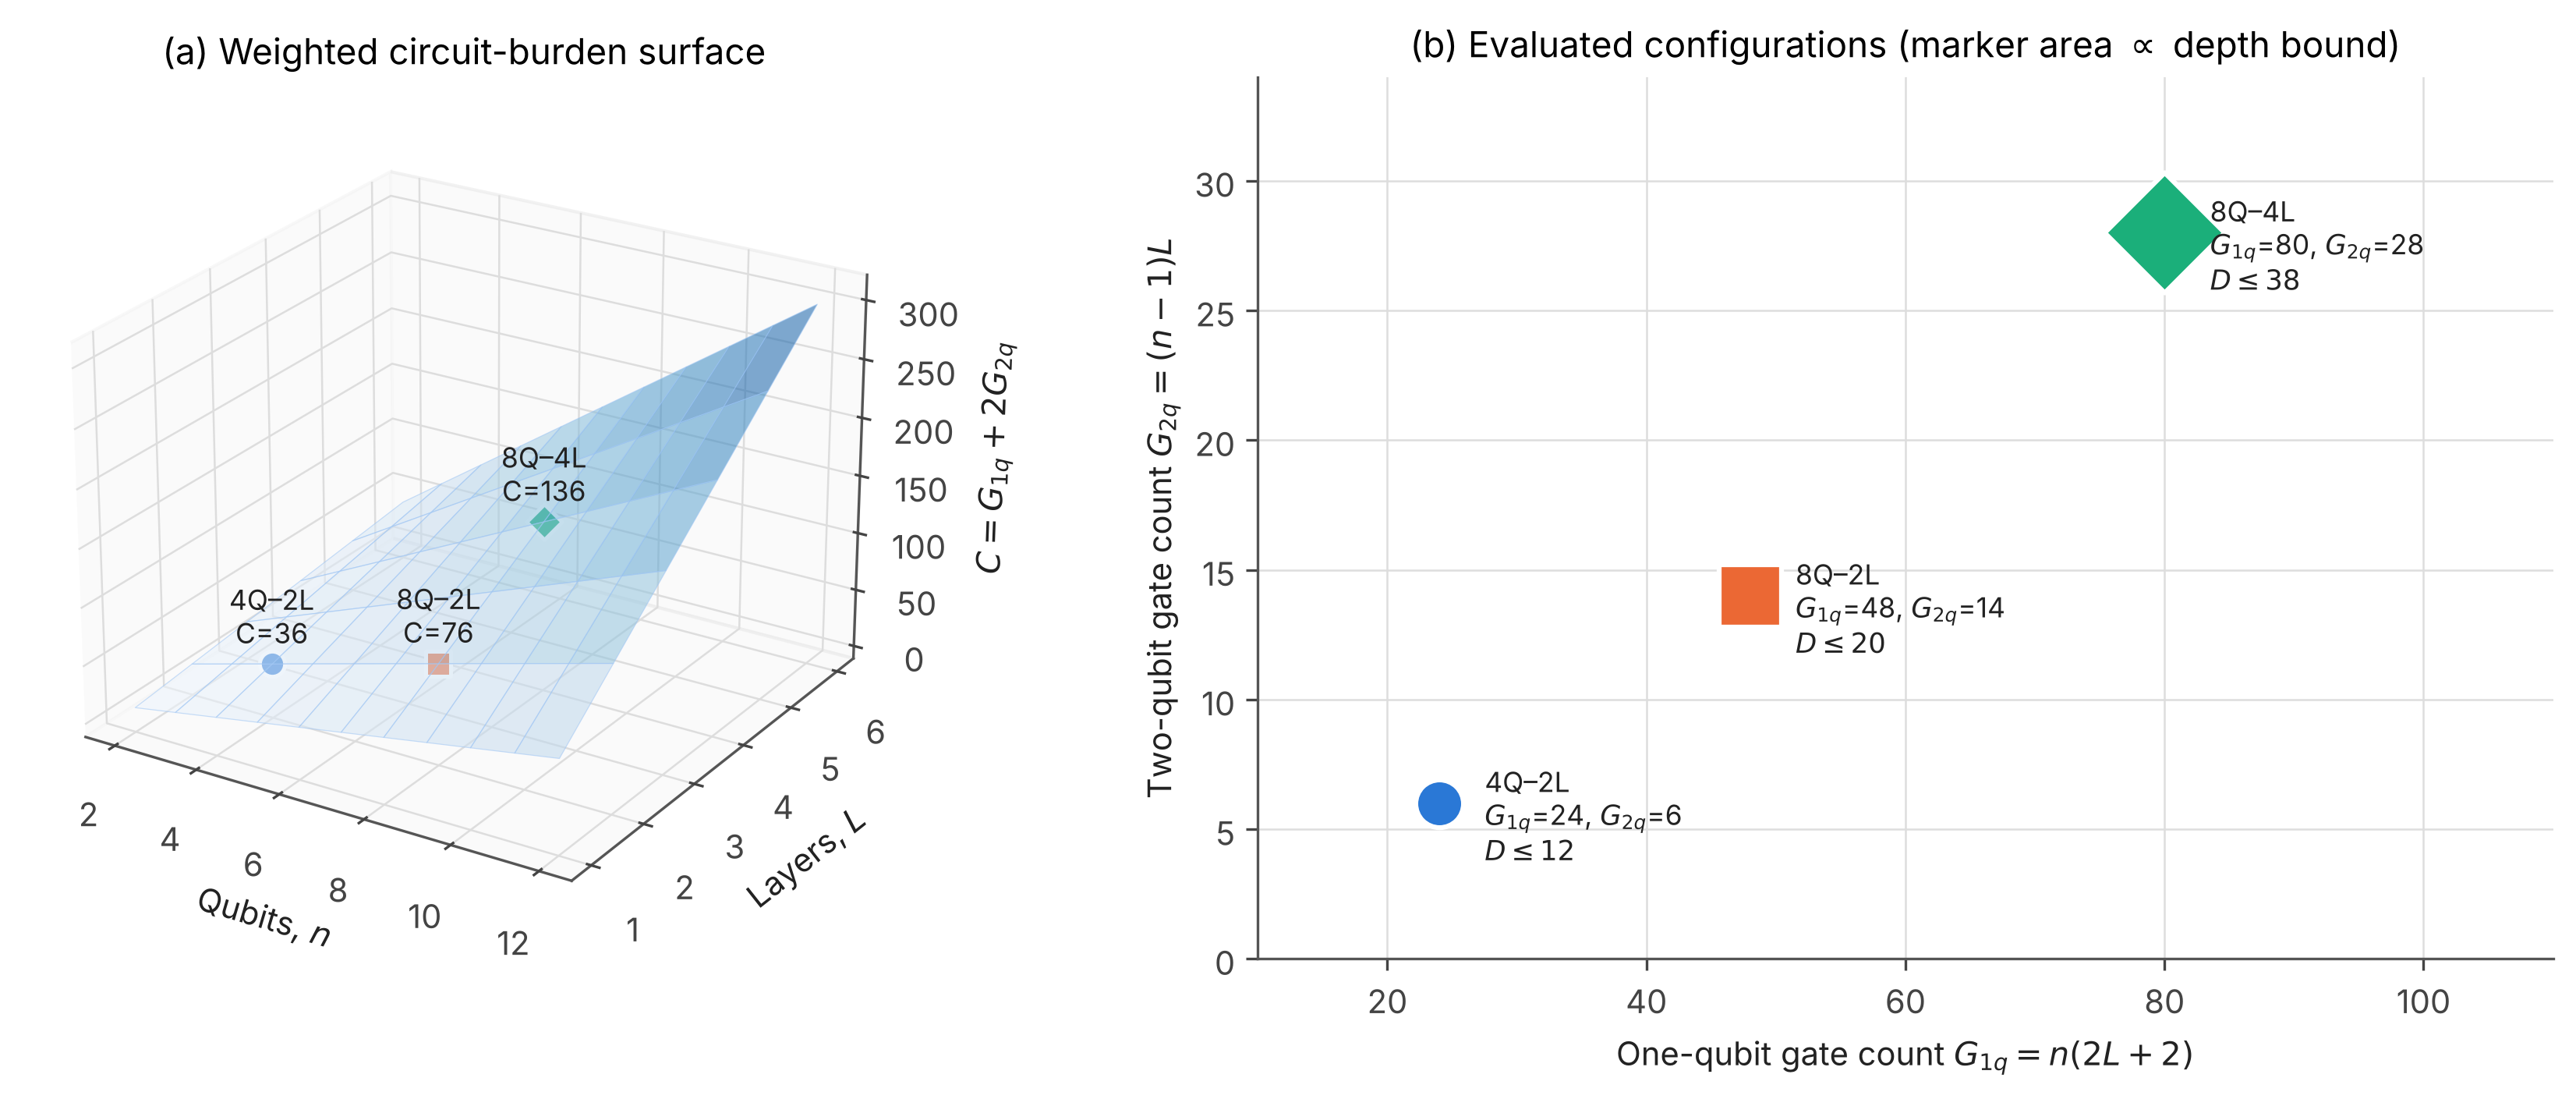
\includegraphics[width=\textwidth]{Figure_4_Complexity_3D (1).png}
  \caption{Analytical circuit burden for the implemented circuit, computed from Eqs.~\eqref{eq:g1q}--\eqref{eq:depth}. Panel (a) presents the weighted circuit burden $C=G_{1q}+2G_{2q}$ as a function of qubit count $n$ and number of layers $L$; the evaluated configurations are marked ($C=36$, $76$, and $136$ for 4Q--2L, 8Q--2L, and 8Q--4L). Panel (b) shows the corresponding one- and two-qubit gate counts, $(G_{1q},G_{2q})=(24,6)$, $(48,14)$, and $(80,28)$, with marker area proportional to the logical-depth upper bound $D\le 2+L(n+1)$ ($12$, $20$, and $38$).}
  \label{fig:complexity_scaling}
\end{figure*}

The analytical gate-survival proxy includes the stated one-qubit error contribution. Figure~\ref{fig:noise_landscape} shows its variation with circuit scale and across the evaluated two-qubit depolarizing error rates.

\begin{figure*}[!tbp]
  \centering
  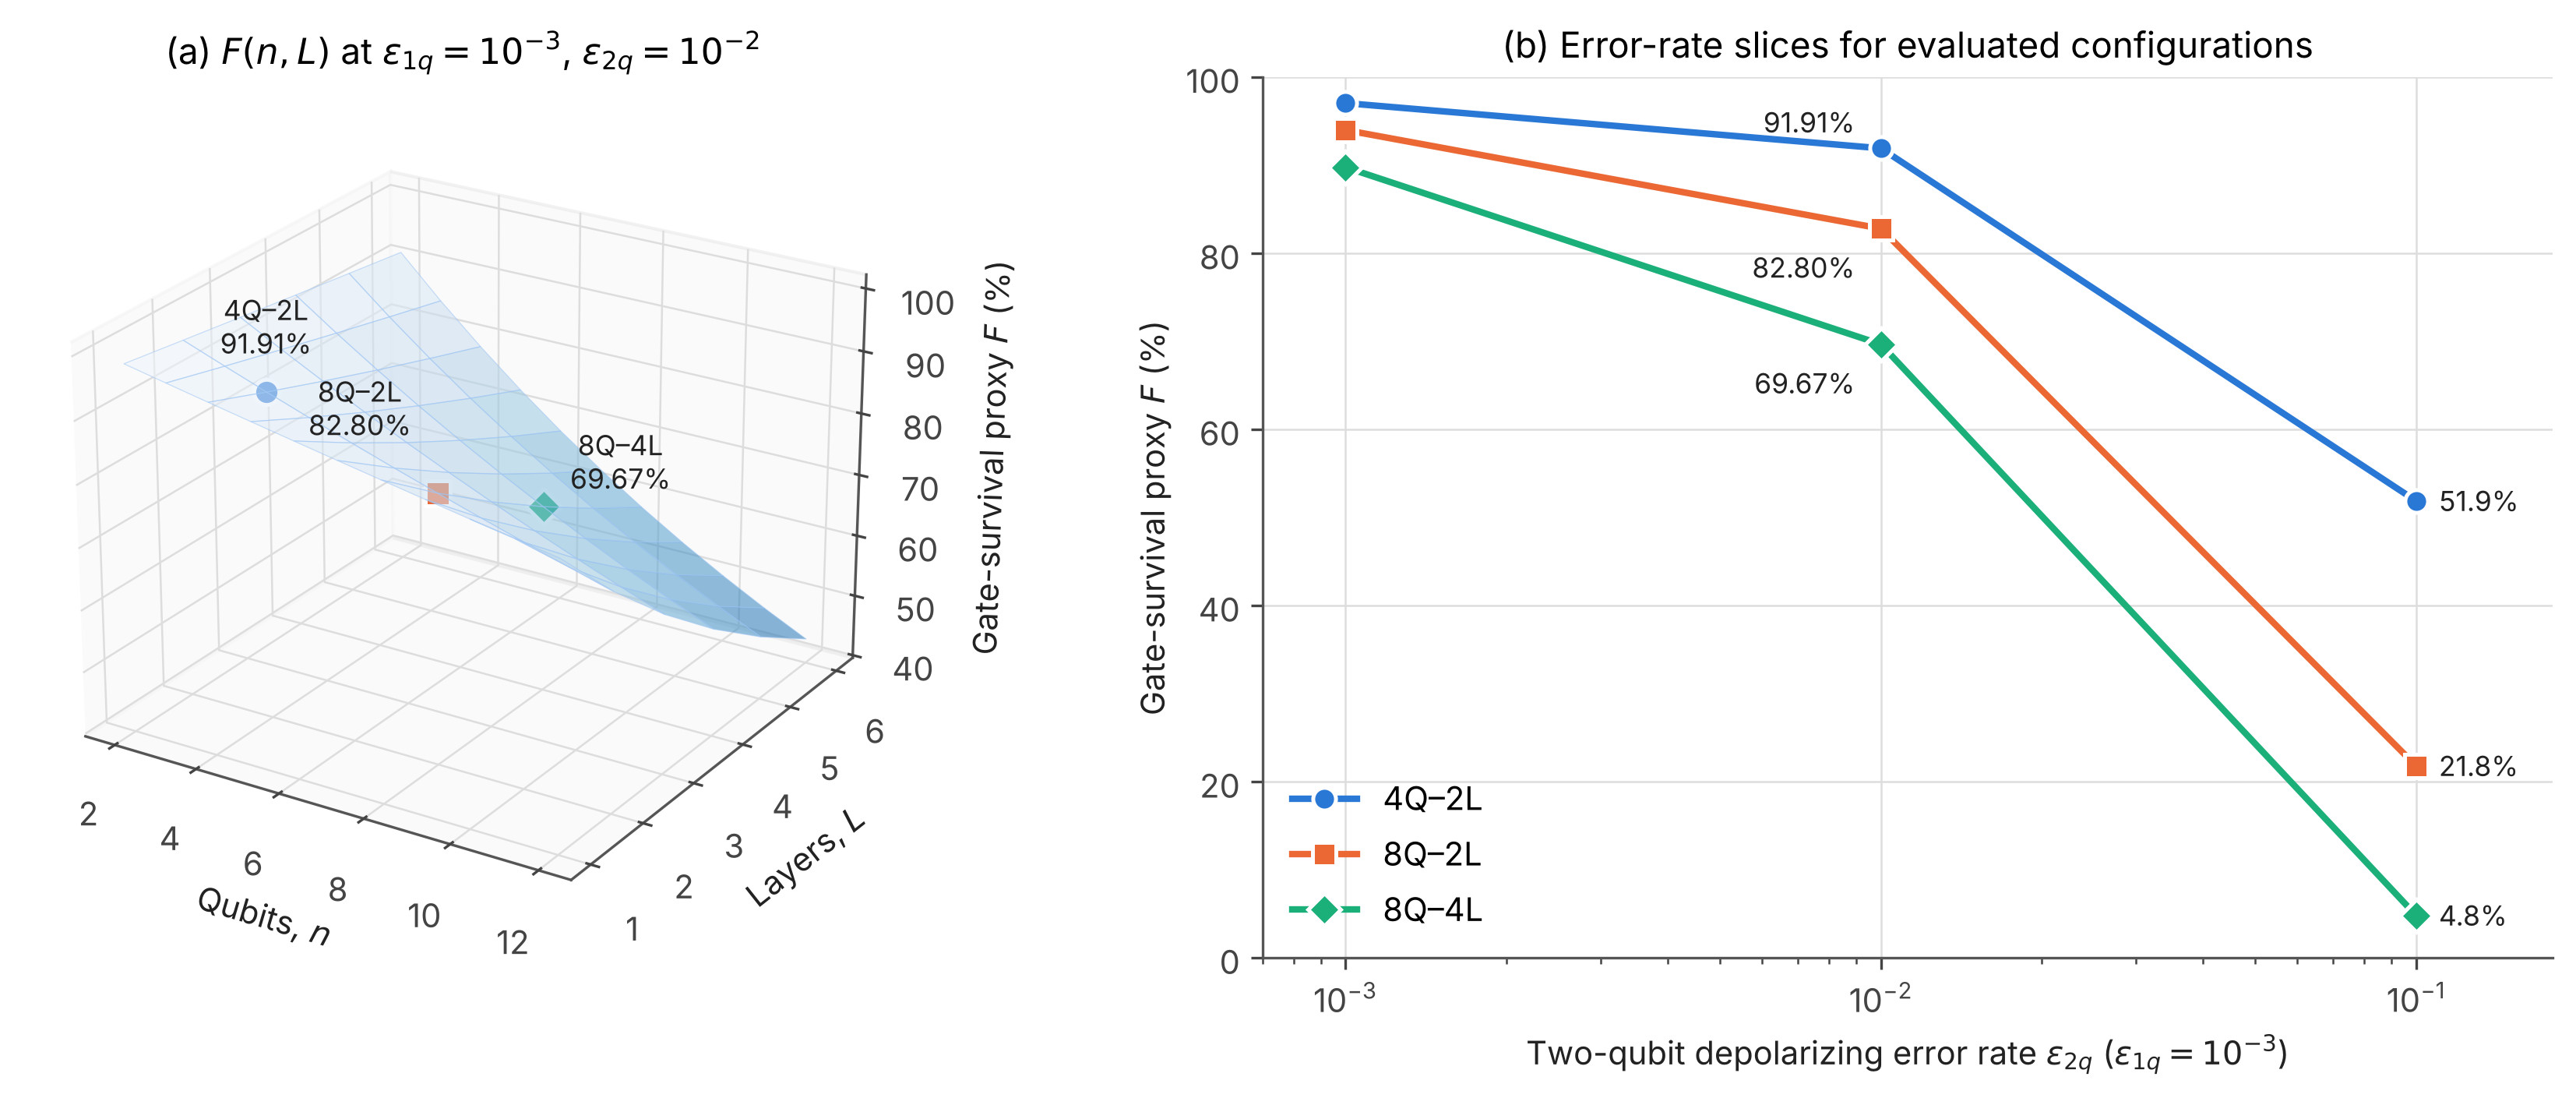
\includegraphics[width=\textwidth]{Figure_5_Noise_3D (1).png}
  \caption{Analytical gate-survival proxy, Eq.~\eqref{eq:fidelity}, for the implemented circuit with $\epsilon_{1q}=10^{-3}$. Panel (a) shows the proxy as a function of qubit count $n$ and number of layers $L$ at $\epsilon_{2q}=10^{-2}$; the evaluated configurations are marked ($91.91\%$, $82.80\%$, and $69.67\%$ for 4Q--2L, 8Q--2L, and 8Q--4L). Panel (b) shows the proxy for the evaluated configurations at $\epsilon_{2q}\in\{10^{-3},10^{-2},10^{-1}\}$.}
  \label{fig:noise_landscape}
\end{figure*}

Table~\ref{tab:classification} reports the secondary classical
five-trial nested cross-validation baseline. The primary
VQC--classical comparison uses the matched evaluation in
Table~\ref{tab:matched_comparison}, where all classical models are
evaluated on the same 15 stratified train/test splits used by the VQC
experiments. Values report mean accuracy, sample standard deviation,
and percentile bootstrap 95\% confidence intervals.

\begin{table*}[!t]
  \centering
  \caption{Secondary Classical Baseline Evaluation Using Five Trials $\times$ Five-Fold Nested Cross-Validation (mean over 25 outer folds; Std.\ is the sample SD of the five repetition means)}
  \label{tab:classification}
  \small
  \begin{tabular}{llcc}
    \toprule
    \textbf{Dataset} & \textbf{Model} & \textbf{Mean accuracy} & \textbf{Std.} \\
    \midrule
    \multirow{6}{*}{Breast Cancer} & Logistic Regression & 0.9656 & 0.0016 \\
    & Linear SVM & 0.9779 & 0.0040 \\
    & SVM (RBF) & 0.9761 & 0.0046 \\
    & Random Forest & 0.9571 & 0.0040 \\
    & MLP & 0.9673 & 0.0109 \\
    & XGBoost & 0.9673 & 0.0098 \\
    \midrule
    \multirow{6}{*}{Binary digits} & Logistic Regression & 1.0000 & 0.0000 \\
    & Linear SVM & 1.0000 & 0.0000 \\
    & SVM (RBF) & 1.0000 & 0.0000 \\
    & Random Forest & 0.9967 & 0.0012 \\
    & MLP & 1.0000 & 0.0000 \\
    & XGBoost & 0.9917 & 0.0034 \\
    \bottomrule
  \end{tabular}
\end{table*}

\begin{table*}[!t]
\centering
\caption{Matched VQC--Classical Performance on Identical 15 Stratified Train/Test Splits. Values report mean accuracy, sample standard deviation, and percentile bootstrap 95\% confidence intervals.}
\label{tab:matched_comparison}
\small
\resizebox{\textwidth}{!}{%
\begin{tabular}{llcccc}
\toprule
\textbf{Dataset} & \textbf{Model} & \textbf{Dimension} &
\textbf{Mean} & \textbf{SD} & \textbf{Bootstrap 95\% CI} \\
\midrule

\multirow{12}{*}{Breast Cancer}
& Logistic Regression & 4 & 0.9345 & 0.0199 & [0.9251, 0.9450] \\
& Linear SVM          & 4 & 0.9439 & 0.0168 & [0.9357, 0.9520] \\
& RBF SVM             & 4 & 0.9509 & 0.0136 & [0.9444, 0.9573] \\
& Random Forest       & 4 & 0.9485 & 0.0140 & [0.9421, 0.9556] \\
& MLP                 & 4 & 0.9544 & 0.0166 & [0.9462, 0.9626] \\
& XGBoost             & 4 & 0.9515 & 0.0172 & [0.9433, 0.9596] \\
& Logistic Regression & 8 & 0.9497 & 0.0211 & [0.9392, 0.9602] \\
& Linear SVM          & 8 & 0.9579 & 0.0141 & [0.9509, 0.9649] \\
& RBF SVM             & 8 & 0.9661 & 0.0128 & [0.9602, 0.9725] \\
& Random Forest       & 8 & 0.9491 & 0.0141 & [0.9427, 0.9567] \\
& MLP                 & 8 & 0.9708 & 0.0135 & [0.9637, 0.9772] \\
& XGBoost             & 8 & 0.9567 & 0.0146 & [0.9497, 0.9637] \\

\midrule

\multirow{12}{*}{Binary digits}
& Logistic Regression & 4 & 0.9972 & 0.0058 & [0.9944, 1.0000] \\
& Linear SVM          & 4 & 0.9972 & 0.0058 & [0.9944, 1.0000] \\
& RBF SVM             & 4 & 1.0000 & 0.0000 & [1.0000, 1.0000] \\
& Random Forest       & 4 & 0.9917 & 0.0102 & [0.9861, 0.9963] \\
& MLP                 & 4 & 0.9972 & 0.0058 & [0.9944, 1.0000] \\
& XGBoost             & 4 & 0.9917 & 0.0115 & [0.9861, 0.9972] \\
& Logistic Regression & 8 & 1.0000 & 0.0000 & [1.0000, 1.0000] \\
& Linear SVM          & 8 & 1.0000 & 0.0000 & [1.0000, 1.0000] \\
& RBF SVM             & 8 & 1.0000 & 0.0000 & [1.0000, 1.0000] \\
& Random Forest       & 8 & 0.9898 & 0.0098 & [0.9852, 0.9944] \\
& MLP                 & 8 & 0.9981 & 0.0049 & [0.9954, 1.0000] \\
& XGBoost             & 8 & 0.9907 & 0.0113 & [0.9852, 0.9963] \\

\bottomrule
\end{tabular}}
\end{table*}

The strongest matched Breast Cancer classical mean is $A_{\mathrm{ref}}=0.9708$ (MLP, $d=8$). The strongest binary-digit mean is $1.0000$; it is attained on every split by the RBF SVM at $d=4$ and by logistic regression, the linear SVM, and the RBF SVM at $d=8$. These values are the accuracy references used in Figure~\ref{fig:performance_landscape}, Table~\ref{tab:paired}, Table~\ref{tab:vdcs_scores}, and Table~\ref{tab:breakeven}. As a trivial reference, a classifier that always predicts the majority training class achieves 0.6316 on every Breast Cancer test partition (72 of 114 test samples are benign) and 0.5000 on every binary-digit test partition.

\begin{table*}[!t]
\centering
\caption{VQC simulation accuracy using 15 independent stratified trials. Values report mean test accuracy, sample standard deviation, and percentile bootstrap 95\% confidence intervals. SPSA uses 20 iterations, 1024 shots, $\epsilon_{1q}=10^{-3}$, and $\epsilon_{2q}=10^{-2}$ during both training and evaluation.}
\label{tab:vqc_accuracy}
\small
\begin{tabular}{lccccc}
\toprule
\textbf{Dataset} & \textbf{$n$} & \textbf{$L$} &
\textbf{Mean} & \textbf{SD} & \textbf{Bootstrap 95\% CI} \\
\midrule
Breast Cancer & 4 & 2 & 0.7409 & 0.1502 & [0.6667, 0.8135] \\
Breast Cancer & 8 & 2 & 0.4474 & 0.2508 & [0.3298, 0.5754] \\
Breast Cancer & 8 & 4 & 0.4848 & 0.2185 & [0.3778, 0.5918] \\
Binary digits & 4 & 2 & 0.5509 & 0.3468 & [0.3815, 0.7167] \\
Binary digits & 8 & 2 & 0.7222 & 0.2769 & [0.5815, 0.8509] \\
Binary digits & 8 & 4 & 0.5417 & 0.2698 & [0.4111, 0.6787] \\
\bottomrule
\end{tabular}
\end{table*}

The highest 15-trial VQC mean is 0.7409 on Breast Cancer (4Q--2L) and
0.7222 on binary digits (8Q--2L); the strongest matched classical means
are 0.9708 and 1.0000. In every configuration, the upper bound of the VQC
percentile-bootstrap 95\% CI (at most 0.8509) lies below the lower bound
of every matched classical CI (at least 0.9251). Because all split-level
outcomes are retained, Table~\ref{tab:paired} also compares each VQC
configuration with the dataset reference split by split. All six mean
paired differences are negative ($-0.5234$ to $-0.2298$) with bootstrap
95\% CIs that exclude zero; the VQC exceeds the reference on only 1 of
the 90 split-level comparisons; and both the paired $t$-test and the
Wilcoxon signed-rank test reject equal accuracy after Holm correction
(adjusted $p\le0.0017$ and $p\le0.0015$, respectively). The two
8-qubit Breast Cancer configurations also fall below the majority-class
rate of 0.6316: their means are 0.4474 and 0.4848, and their CI upper
bounds are 0.5754 and 0.5918. All binary-digit means exceed 0.5, but the
CIs for 4Q--2L and 8Q--4L include 0.5.
Figure~\ref{fig:performance_landscape} visualizes the split-level VQC
results, the matched classical references, and the majority-class rates.

\begin{table*}[!t]
\centering
\caption{Paired VQC--classical comparison on identical splits ($\epsilon_{2q}=10^{-2}$). The difference is VQC accuracy minus reference accuracy on the same split; ``VQC wins'' counts splits on which the VQC is strictly more accurate. $p$-values are Holm-adjusted over the six comparisons.}
\label{tab:paired}
\small
\begin{tabular}{lcclccccc}
\toprule
\textbf{Dataset} & \textbf{$n$} & \textbf{$L$} & \textbf{Reference} & \textbf{Mean diff.} & \textbf{Bootstrap 95\% CI} & \textbf{VQC wins} & \textbf{$p$ (paired $t$)} & \textbf{$p$ (Wilcoxon)} \\
\midrule
Breast Cancer & 4 & 2 & MLP ($d=8$) & $-0.2298$ & [$-0.3035$, $-0.1579$] & 1/15 & $1.1\times10^{-4}$ & $3.7\times10^{-4}$ \\
Breast Cancer & 8 & 2 & MLP ($d=8$) & $-0.5234$ & [$-0.6415$, $-0.3947$] & 0/15 & $6.9\times10^{-6}$ & $3.7\times10^{-4}$ \\
Breast Cancer & 8 & 4 & MLP ($d=8$) & $-0.4860$ & [$-0.5895$, $-0.3825$] & 0/15 & $2.7\times10^{-6}$ & $3.7\times10^{-4}$ \\
Binary digits & 4 & 2 & RBF SVM ($d=4$) & $-0.4491$ & [$-0.6250$, $-0.2815$] & 0/15 & $3.8\times10^{-4}$ & $3.7\times10^{-4}$ \\
Binary digits & 8 & 2 & RBF SVM ($d=4$) & $-0.2778$ & [$-0.4213$, $-0.1519$] & 0/15 & $1.6\times10^{-3}$ & $1.5\times10^{-3}$ \\
Binary digits & 8 & 4 & RBF SVM ($d=4$) & $-0.4583$ & [$-0.5889$, $-0.3287$] & 0/15 & $4.9\times10^{-5}$ & $3.7\times10^{-4}$ \\
\bottomrule
\end{tabular}
\end{table*}

These accuracies characterize the VQC under the specified optimization
budget rather than the best accuracy the ansatz can reach. With the gains
of Algorithm~\ref{alg:vqc}, the SPSA step coefficient $a_k$ decreases
from 0.0118 to 0.0065 over the 20 iterations, and the SPSA loss estimate
falls by 16.1\% on average between the first and the last iteration
(per-configuration means 7.9--27.8\%). The final parameters therefore
remain close to their random initialization
$\boldsymbol{\theta}\sim\mathcal{U}(-\pi,\pi)^P$. Across the 90 primary
trials, train and test accuracy are almost perfectly correlated (Pearson
$r=0.992$), and 35 of the 90 trials have test accuracy below 0.5, which
indicates a sign-inverted decision rule inherited from the initial
parameters. The large split-to-split standard deviations in
Table~\ref{tab:vqc_accuracy} (0.150--0.347) reflect this initialization
dependence more than data-split variation. A larger iteration budget
or tuned SPSA gains would be expected to raise the VQC accuracies, so the
comparison above is a comparison under the stated 20-iteration budget.

\begin{figure*}[!tbp]
  \centering
  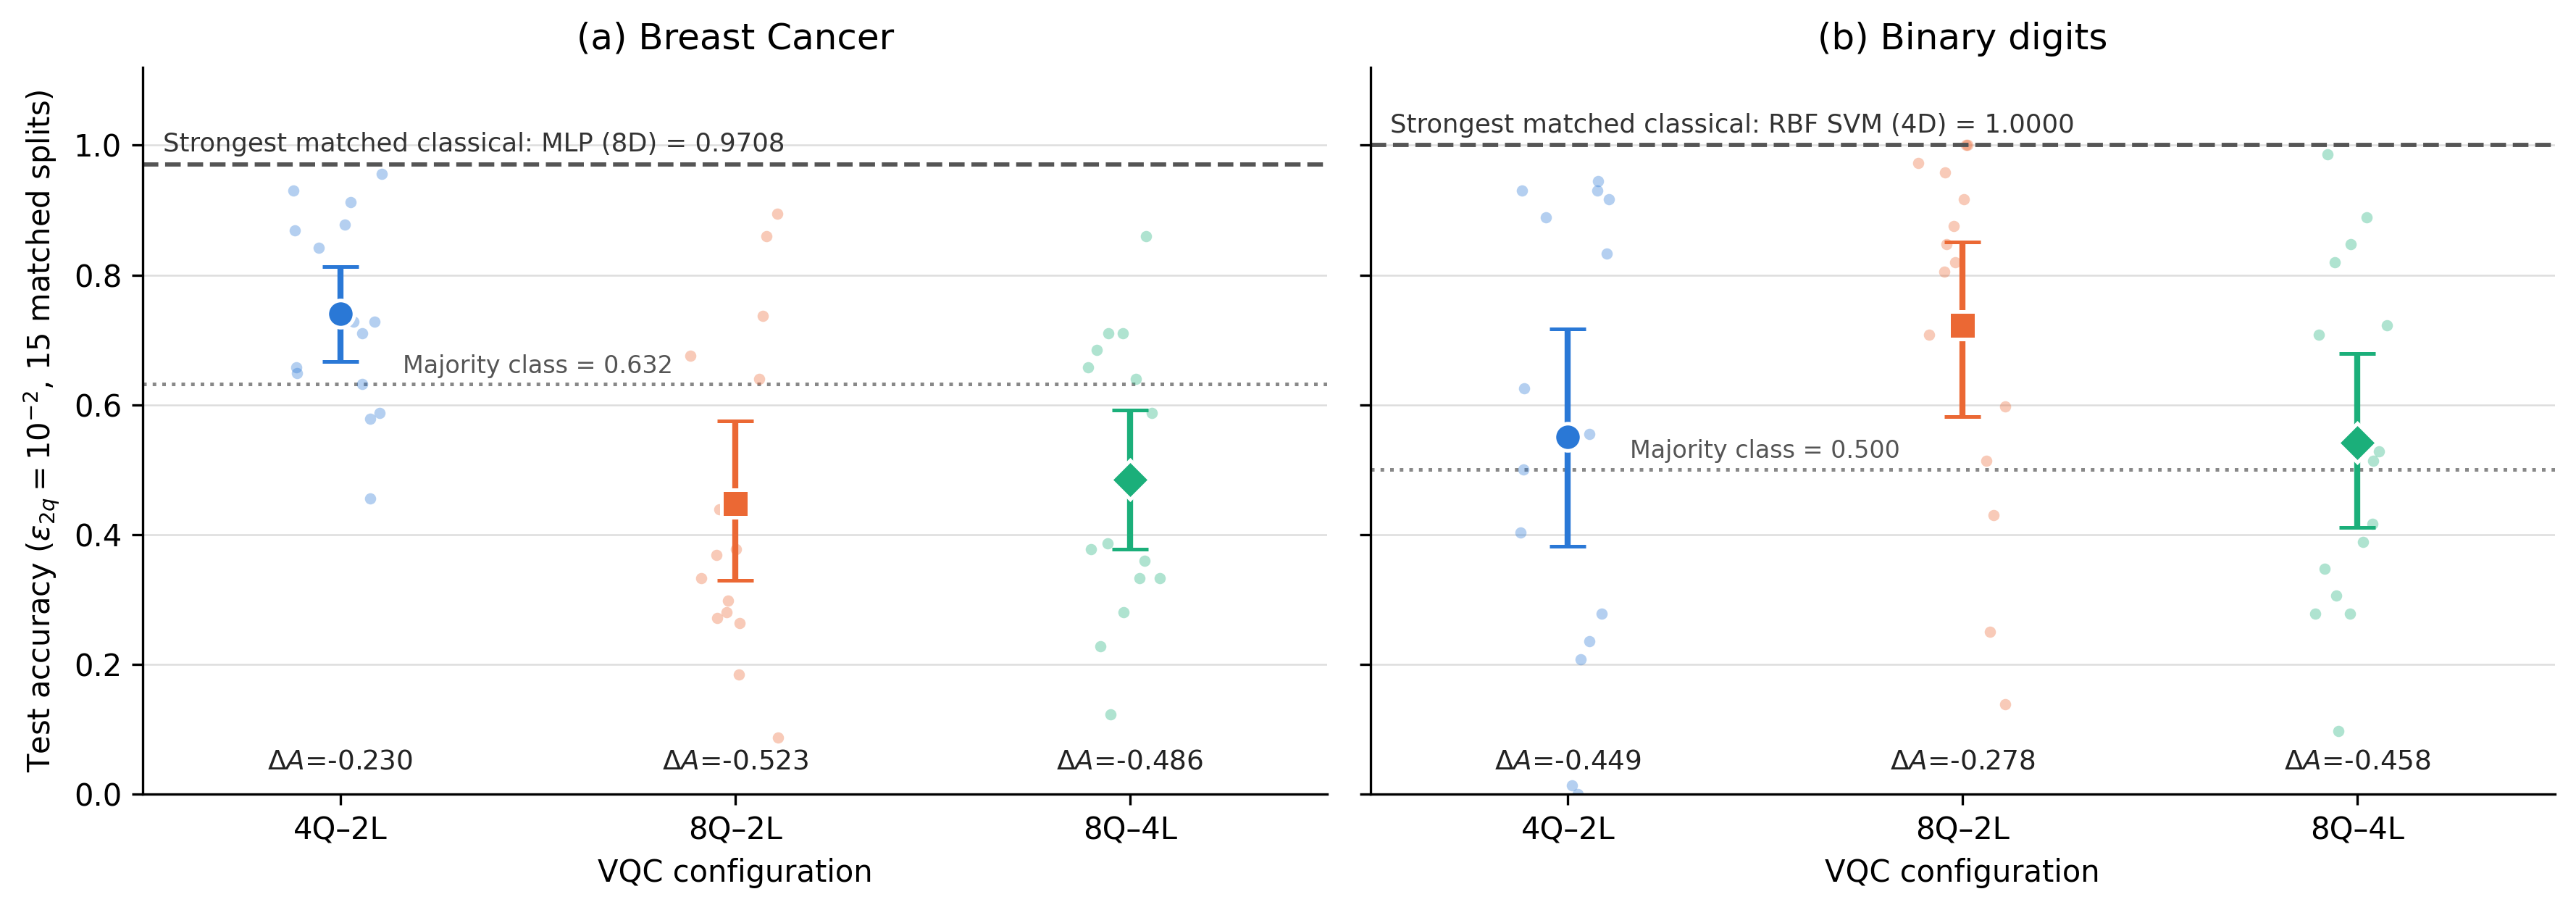
\includegraphics[width=\textwidth]{Figure_6_Performance_Landscape 1.png}
  \caption{Matched VQC--classical performance comparison on the same 15 independent stratified train/test splits ($\epsilon_{2q}=10^{-2}$). Panels (a) Breast Cancer and (b) binary digits show mean VQC test accuracy (large markers) with percentile bootstrap 95\% confidence intervals and the 15 split-level accuracies (small points) for each evaluated configuration (4Q--2L, 8Q--2L, 8Q--4L). The dashed line is the strongest matched classical mean for that dataset ($0.9708$ for Breast Cancer, $1.0000$ for binary digits), the dotted line is the majority-class rate (0.632 and 0.500), and the annotation gives $\Delta A=A_{\mathrm{VQC}}-A_{\mathrm{ref}}$.}
  \label{fig:performance_landscape}
\end{figure*}

Table~\ref{tab:noise_sensitivity} reports noise sensitivity on the same 15 splits under two protocols. In the fixed-model protocol, the parameters trained at $\epsilon_{2q}=10^{-2}$ are re-evaluated without retraining at $\epsilon_{2q}\in\{10^{-3},10^{-2},10^{-1}\}$. In the retrained protocol, Algorithm~\ref{alg:vqc} is rerun at each noise level from the same split-seeded initialization; its $\epsilon_{2q}=10^{-2}$ column is Table~\ref{tab:vqc_accuracy}. The fixed-model means change by at most 0.006 across the hundred-fold range of $\epsilon_{2q}$, although the analytical proxy for 8Q--4L falls from 89.76\% to 4.83\% over the same range. The decision rule uses only the sign of $\langle Z_0\rangle$, and depolarizing noise mainly contracts its magnitude, so predictions rarely change. The retrained means vary by 0.016--0.061, which is well within the split-to-split standard deviation. Under the 20-iteration budget, the noise level therefore affects accuracy much less than the parameter initialization does. The fixed-model and retrained values at $\epsilon_{2q}=10^{-2}$ use the same parameters and differ only through shot-sampling randomness.

\begin{table*}[!t]
  \centering
  \caption{Noise sensitivity over the 15 matched splits (mean $\pm$ sample SD of test accuracy; $\epsilon_{1q}=10^{-3}$). Fixed model: parameters trained at $\epsilon_{2q}=10^{-2}$ and evaluated at each $\epsilon_{2q}$. Retrained: Algorithm~\ref{alg:vqc} rerun at each $\epsilon_{2q}$.}
  \label{tab:noise_sensitivity}
  \small
  \resizebox{\textwidth}{!}{%
  \begin{tabular}{lcccccccc}
    \toprule
    & & & \multicolumn{3}{c}{\textbf{Fixed model}} & \multicolumn{3}{c}{\textbf{Retrained}} \\
    \cmidrule(lr){4-6}\cmidrule(lr){7-9}
    \textbf{Dataset} & \textbf{$n$} & \textbf{$L$} & \textbf{$10^{-3}$} & \textbf{$10^{-2}$} & \textbf{$10^{-1}$} & \textbf{$10^{-3}$} & \textbf{$10^{-2}$} & \textbf{$10^{-1}$} \\
    \midrule
    Breast Cancer & 4 & 2 & 0.734 $\pm$ 0.154 & 0.738 $\pm$ 0.154 & 0.737 $\pm$ 0.152 & 0.750 $\pm$ 0.144 & 0.741 $\pm$ 0.150 & 0.721 $\pm$ 0.174 \\
    Breast Cancer & 8 & 2 & 0.442 $\pm$ 0.245 & 0.446 $\pm$ 0.246 & 0.444 $\pm$ 0.246 & 0.463 $\pm$ 0.236 & 0.447 $\pm$ 0.251 & 0.449 $\pm$ 0.242 \\
    Breast Cancer & 8 & 4 & 0.477 $\pm$ 0.217 & 0.480 $\pm$ 0.215 & 0.481 $\pm$ 0.216 & 0.495 $\pm$ 0.222 & 0.485 $\pm$ 0.219 & 0.459 $\pm$ 0.222 \\
    Binary digits & 4 & 2 & 0.549 $\pm$ 0.342 & 0.553 $\pm$ 0.338 & 0.551 $\pm$ 0.339 & 0.556 $\pm$ 0.348 & 0.551 $\pm$ 0.347 & 0.503 $\pm$ 0.346 \\
    Binary digits & 8 & 2 & 0.724 $\pm$ 0.280 & 0.719 $\pm$ 0.286 & 0.725 $\pm$ 0.282 & 0.732 $\pm$ 0.251 & 0.722 $\pm$ 0.277 & 0.671 $\pm$ 0.303 \\
    Binary digits & 8 & 4 & 0.539 $\pm$ 0.273 & 0.535 $\pm$ 0.272 & 0.540 $\pm$ 0.278 & 0.554 $\pm$ 0.268 & 0.542 $\pm$ 0.270 & 0.506 $\pm$ 0.282 \\
    \bottomrule
  \end{tabular}}
\end{table*}

Figure~\ref{fig:noise_sensitivity} shows the fixed-model accuracy matrix and the sensitivity amplitudes of both protocols.

\begin{figure*}[!tbp]
  \centering
  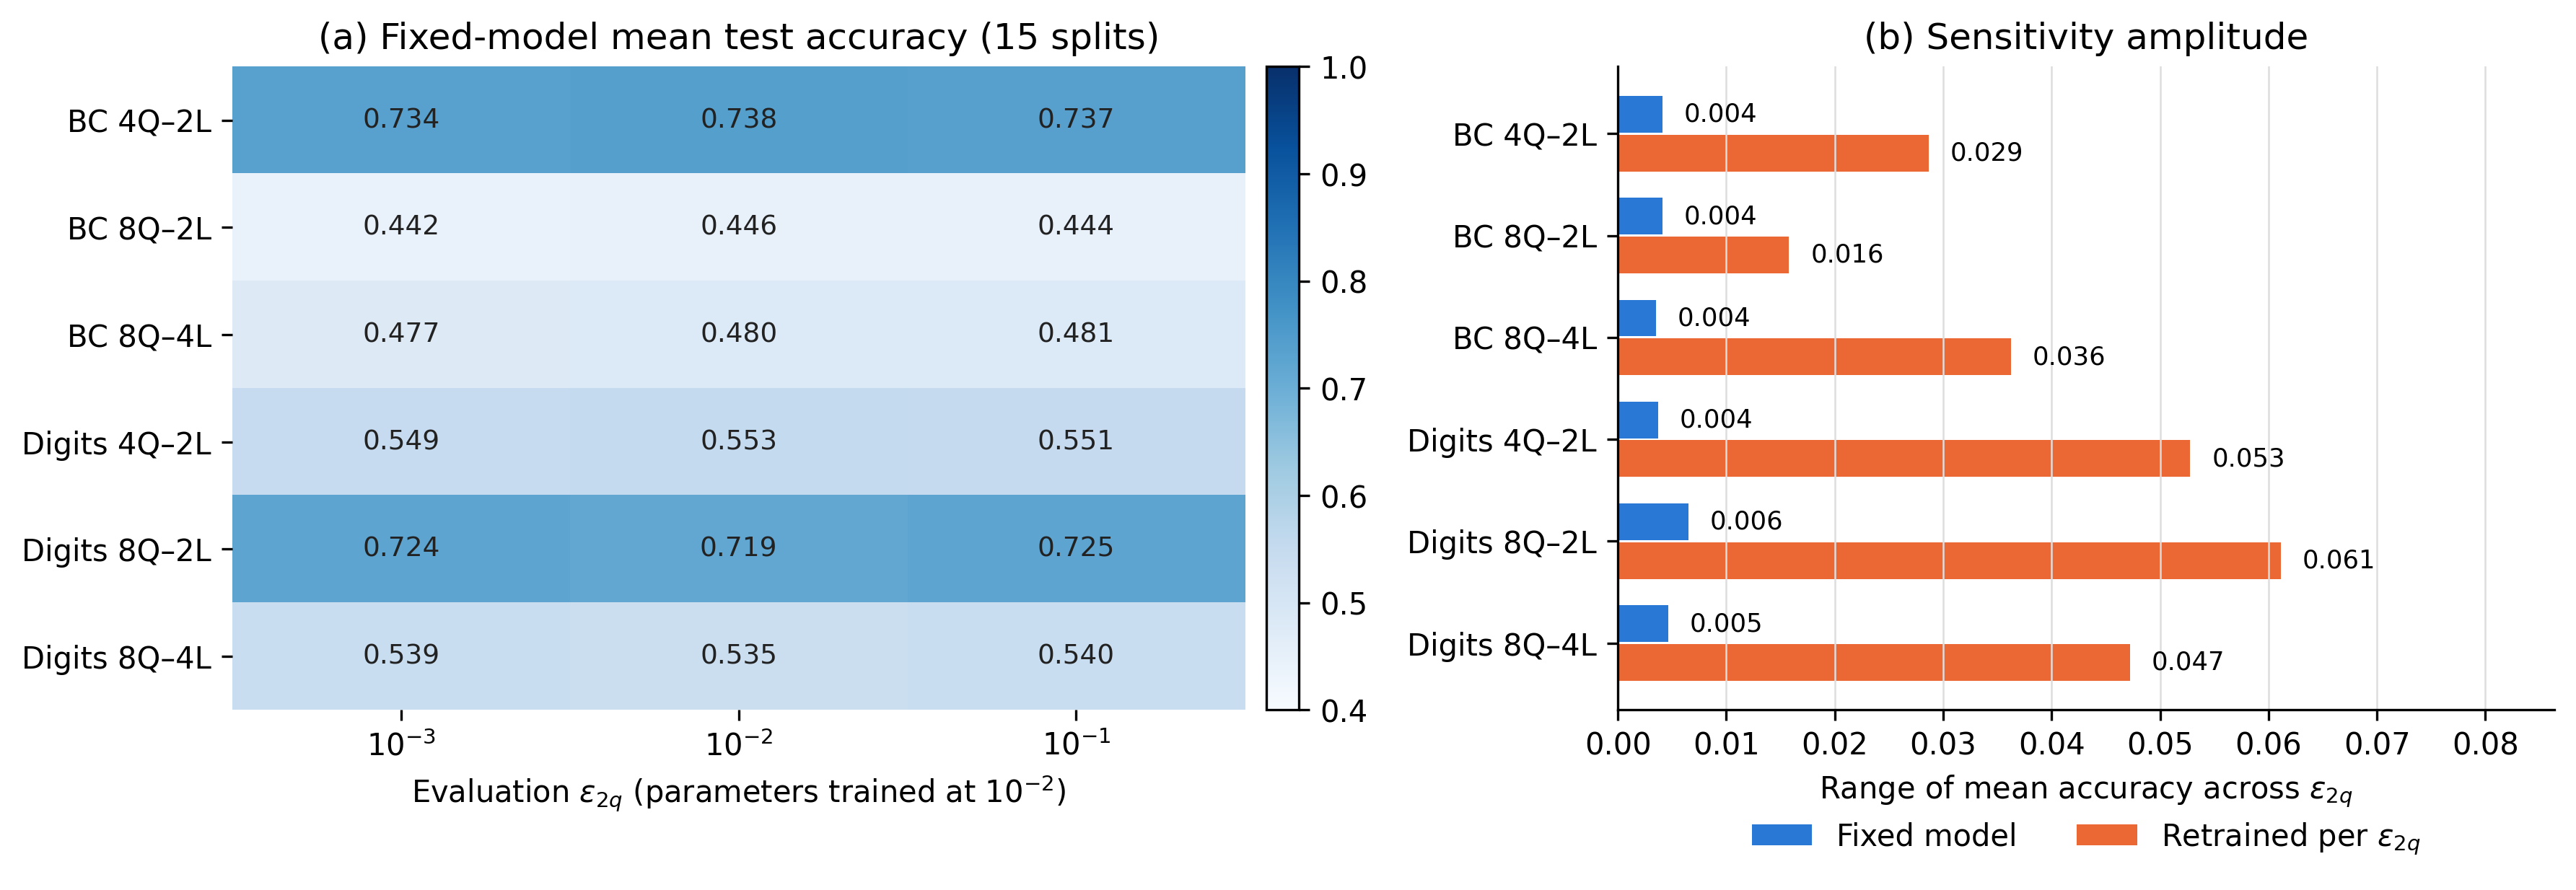
\includegraphics[width=\textwidth]{Figure_7_Noise_Sensitivity.png}
  \caption{Noise sensitivity over the 15 matched splits. Panel (a) shows the fixed-model mean test accuracy for parameters trained at $\epsilon_{2q}=10^{-2}$ and evaluated at the three two-qubit depolarizing error rates. Panel (b) shows the sensitivity amplitude, the range between the largest and smallest mean accuracy across the three error rates, for the fixed-model and retrained protocols.}
  \label{fig:noise_sensitivity}
\end{figure*}

\subsection{Local Aer Compilation and Execution Timing}
\label{sec:latency}

Table~\ref{tab:latency} reports local Aer compilation and execution wall-clock time for 20 circuits of the final architecture in Figure~\ref{fig:vqc_ansatz}, measured as described in Section~\ref{sec:methodology} (pathway (ii)). The execution share is $T_{\mathrm{exec}}/(T_{\mathrm{compile}}+T_{\mathrm{exec}})$. Transpilation onto the linear coupling map inserts no SWAP gates: the transpiled circuits contain exactly $G_{2q}=6$, 14, and 28 CX gates, with depths 14, 18, and 30. Aer selects its density-matrix method for these noisy circuits. At this scale, compilation dominates local cost. Execution accounts for only 8.3--11.1\% of compile-plus-execution time, and the total time grows by a factor of 1.77 (0.503\,s to 0.889\,s) while the weighted burden $C$ grows by a factor of 3.8 (36 to 136). This timing scope covers local compilation and execution only. End-to-end latency also includes preprocessing, optimization, networking, queueing, QPU execution, and classical-baseline timing. The timing values enter only the $s_T$ component of the Pre-VDCS.

\begin{table*}[!t]
  \centering
  \caption{Local Aer Simulator Wall-Clock Timing (20 Circuits per Configuration)}
  \label{tab:latency}
  \small
  \setlength{\tabcolsep}{3pt}
    \begin{tabular}{ccccccc}
      \toprule
      \textbf{Qubits} & \textbf{Layers} & \textbf{Compile (s)} & \textbf{Execution (s)} & \textbf{Execution share (\%)} & \textbf{Transpiled depth} & \textbf{CX count} \\
      \midrule
      4 & 2 & 0.461 $\pm$ 0.030 & 0.042 $\pm$ 0.006 & 8.3 & 14 & 6 \\
      8 & 2 & 0.596 $\pm$ 0.021 & 0.054 $\pm$ 0.002 & 8.3 & 18 & 14 \\
      8 & 4 & 0.790 $\pm$ 0.047 & 0.099 $\pm$ 0.003 & 11.1 & 30 & 28 \\
      \bottomrule
    \end{tabular}
  \begin{tablenotes}
    \small
  \item Mean $\pm$ sample SD over ten timed repetitions (after one warm-up) on a 4-vCPU Intel Xeon (2.00\,GHz) Linux virtual machine. Execution share = execution/(compile + execution) $\times 100$, averaged over repetitions. All values are local Qiskit Aer wall-clock measurements, separate from the Pauli-propagation simulator used for the primary accuracy results. Cloud, queue, QPU, and end-to-end training timing require separate measurements.
  \end{tablenotes}
\end{table*}

Figure~\ref{fig:runtime_burden} relates the reported weighted circuit burden to the local compile-plus-execution wall-clock measurements and execution shares.

\begin{figure*}[!tbp]
  \centering
  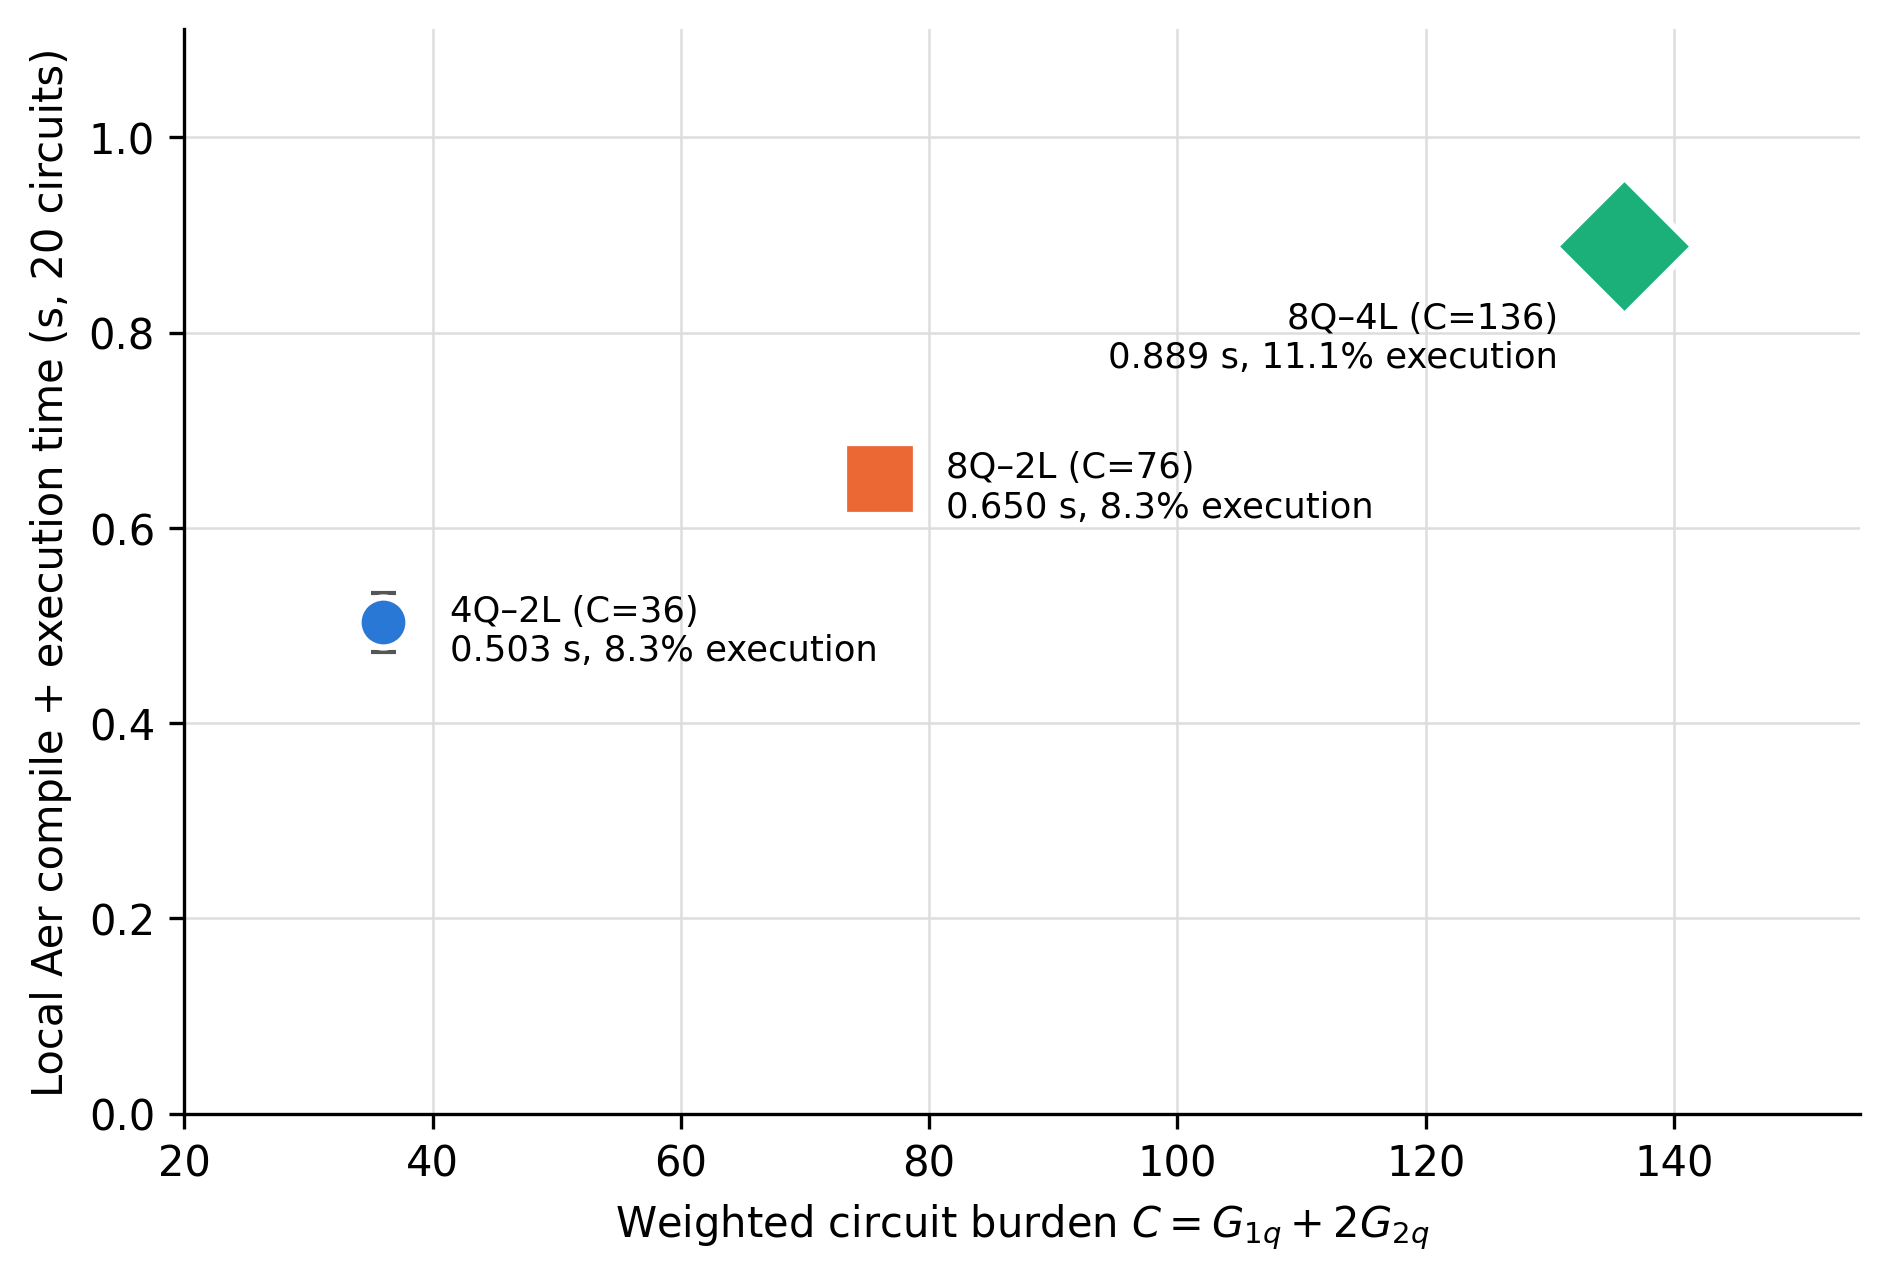
\includegraphics[width=0.50\textwidth]{Figure_8_Runtime_Burden (1).png}
  \caption{Relationship between circuit burden and local execution cost. The horizontal axis is the analytical weighted circuit burden $C=G_{1q}+2G_{2q}$ of the implemented circuit ($36$, $76$, and $136$), and the vertical axis is the measured local Qiskit Aer compile-plus-execution wall-clock time for 20 circuits from Table~\ref{tab:latency}. Marker area is proportional to $C$, error bars show the combined sample SD of compile and execution time over ten repetitions, and the annotation gives the total time and execution share.}
  \label{fig:runtime_burden}
\end{figure*}

% =================================================
\section{Offline Backend-Calibrated Simulation Check}
\label{sec:hardware}
% =================================================

The backend-calibrated check uses an offline \texttt{FakeNairobiV2} snapshot. It uses Breast Cancer with $n=4$ and $L=2$ on the same 15 splits as the primary experiment (Section~\ref{sec:methodology}, pathway (iii)); SABRE maps the four logical qubits to physical qubits $[4,5,3,1]$. This is a local simulator experiment. Its evidence scope is the backend-derived calibration snapshot. Live \texttt{ibm\_nairobi} experiments can measure queue time, QPU execution time, calibration drift, qubit-layout selection, and error-mitigation performance.

\begin{table}[!htbp]
  \centering
  \caption{Offline FakeNairobiV2 Calibrated-Model Check (Breast Cancer; $n=4$, $L=2$; 15 splits)}
  \label{tab:hardware_comparison}
  \small
  \setlength{\tabcolsep}{4pt}
  \begin{tabular}{lc}
    \toprule
    \textbf{Quantity} & \textbf{Value} \\
    \midrule
    Test accuracy (mean $\pm$ SD) & $0.7216\pm0.1691$ \\
    Bootstrap 95\% CI of mean & [0.6368, 0.8029] \\
    Range over splits & 0.3596--0.9474 \\
    Synthetic model (Table~\ref{tab:vqc_accuracy}) & $0.7409\pm0.1502$ \\
    Paired difference & $-0.0193$ \\
    \quad bootstrap 95\% CI & [$-0.0392$, $-0.0029$] \\
    \quad Wilcoxon $p$ & 0.090 \\
    Training time per split (s) & $34.75\pm0.28$ \\
    Test evaluation per split (s) & $0.277\pm0.027$ \\
    \bottomrule
  \end{tabular}
  \begin{tablenotes}
    \small
    \item SD is the sample SD over 15 splits. Paired difference is calibrated minus synthetic accuracy on the same split. Times are local wall-clock values.
  \end{tablenotes}
\end{table}

Over the 15 splits, the calibrated-snapshot model gives mean test accuracy 0.7216 (sample SD 0.1691). The split-level accuracies closely track those of the primary synthetic depolarizing model (Figure~\ref{fig:calibrated_variability}a). The mean paired difference is $-0.0193$; its bootstrap 95\% CI only just excludes zero, and the Wilcoxon signed-rank test does not reject equality ($p=0.090$). The calibrated noise model therefore lowers accuracy by about 0.02 on average relative to the synthetic model (bootstrap 95\% CI 0.003--0.039). Both pathways start from the same split-seeded initial parameters, so this agreement is consistent with the initialization-dominated regime described in Section~\ref{sec:experiments}. Training on the calibrated model, with every loss evaluation estimated from 1024 Aer shots, takes $34.75\pm0.28$\,s per split, and test evaluation takes $0.277\pm0.027$\,s. These are local simulator costs on the machine described in Section~\ref{sec:methodology}, not QPU or queue times. Live-hardware and cloud-service timing require a separate experiment.

\begin{figure*}[!tbp]
  \centering
  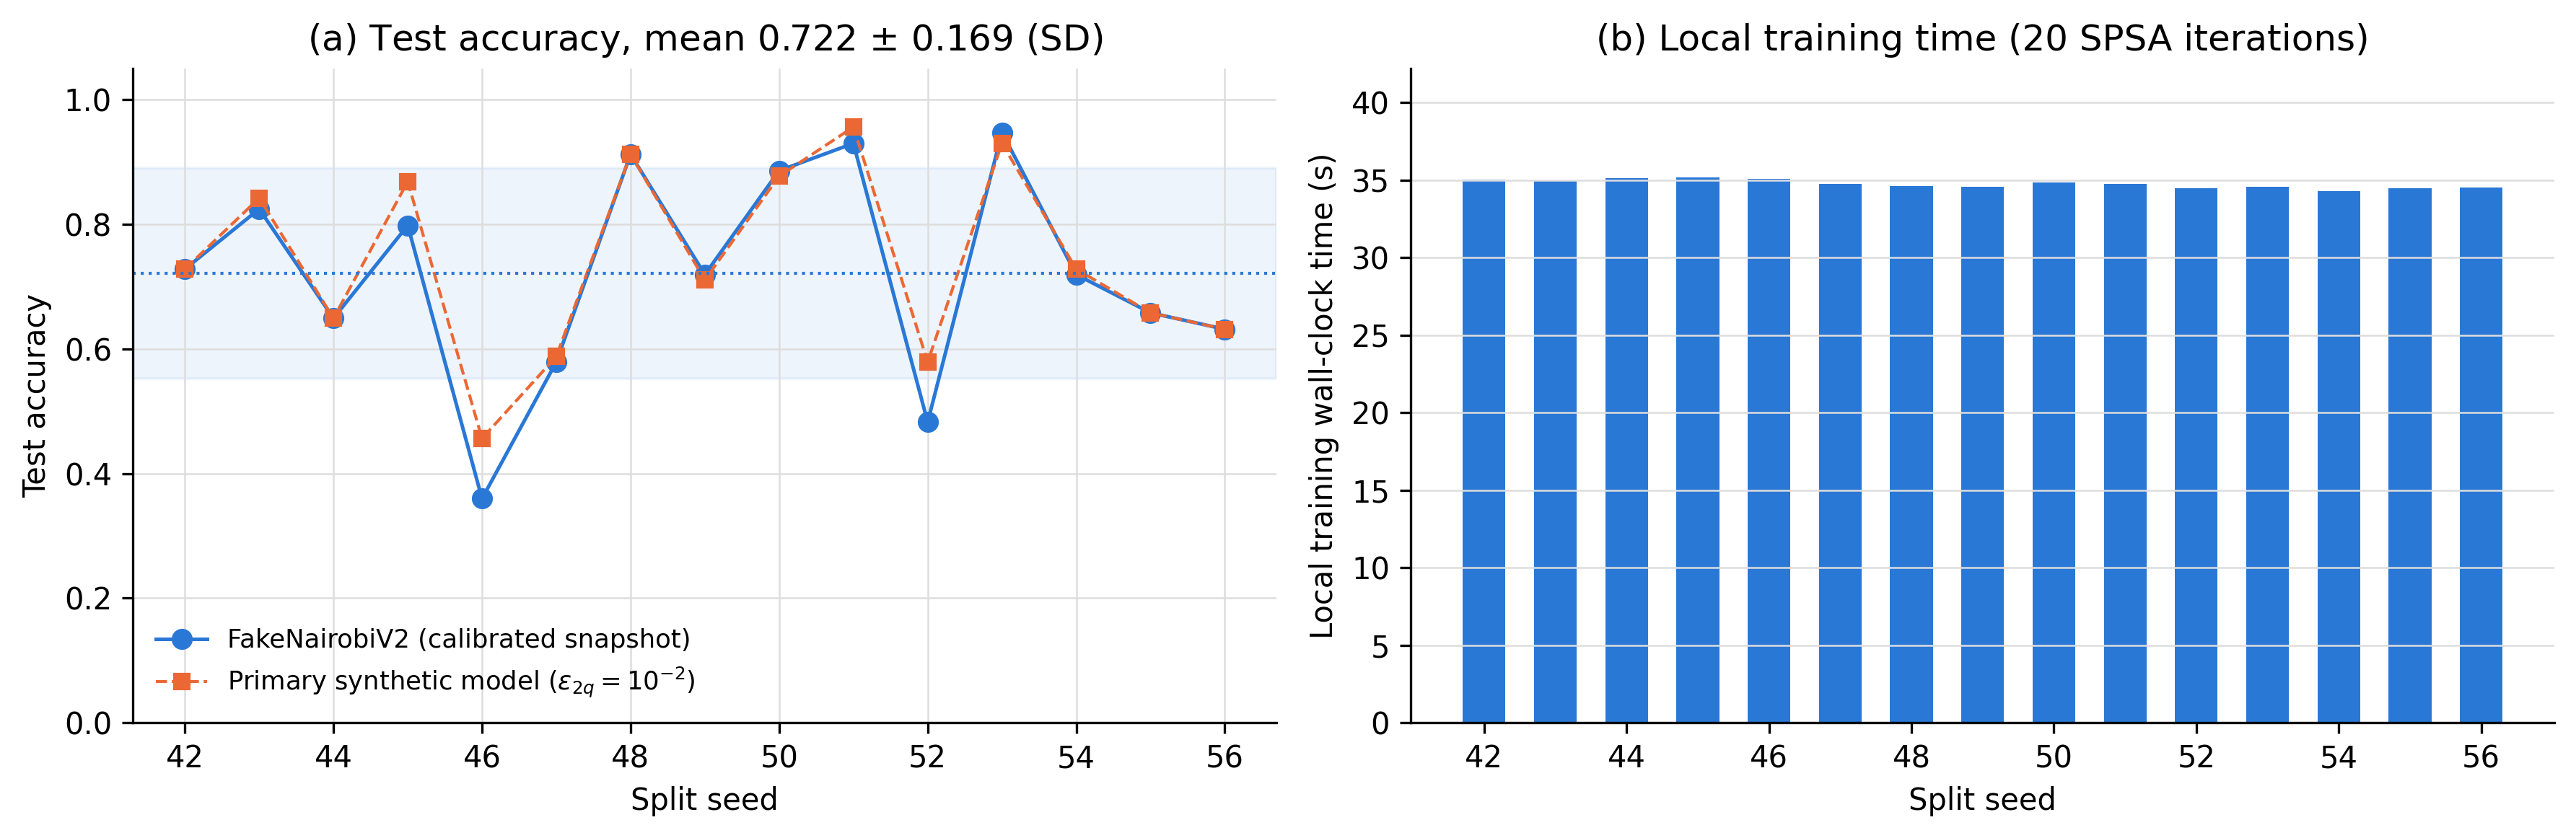
\includegraphics[width=\textwidth]{Figure_9_Calibrated_Model 1.png}
  \caption{Offline backend-calibrated simulation using the FakeNairobiV2 snapshot for Breast Cancer classification with $n=4$ and $L=2$ on the 15 matched splits. Panel (a) shows split-level test accuracy under the calibrated model (circles) and under the primary synthetic depolarizing model at $\epsilon_{2q}=10^{-2}$ (squares), with the calibrated-model mean (dotted line) and $\pm1$ sample SD band. Panel (b) reports the local training wall-clock time per split.}
  \label{fig:calibrated_variability}
\end{figure*}

% =================================================
\section{System-Level VQC Deployment Evaluation}
\label{sec:readiness}
% =================================================

\label{sec:vdcs}

We introduce a \emph{Pre-Deployment VQC Competitiveness
Score} (Pre-VDCS) as a study-scoped multi-criteria index. It ranks VQC
configurations using quantities directly measured or derived from the
present simulation study. The Pre-VDCS uses classification accuracy,
local compile-plus-execution time, analytical noise-robustness, and
circuit-evaluation burden. It does not represent live deployment
performance. The full VDCS requires additional measurements from live
QPU execution, queueing, mitigation, energy, and cost.

For configuration $c$, $A_c$ is mean accuracy, $T_c$ is local
compile-plus-execution time, $F_c$ is the analytical gate-survival
noise-robustness proxy, and $C_c$ is the circuit-evaluation burden.
$A_{\mathrm{ref}}$ is the strongest matched classical accuracy for the
same dataset. $T_0$ is the fastest measured local compile-plus-execution
time among the evaluated configurations, and $C_0$ is the corresponding baseline
circuit burden. Because no mitigation procedure is evaluated in the
present experiments, the Pre-VDCS contains no mitigation component.
\begin{align}
s_A(c) &= \min\!\left\{1,\frac{A_c}{A_{\mathrm{ref}}}\right\}, &
s_T(c) &= \min\!\left\{1,\frac{T_0}{T_c}\right\}, \label{eq:vdcs_components}\\
s_N(c) &= F_c, &
s_C(c) &= \min\!\left\{1,\frac{C_0}{C_c}\right\}, \nonumber\\
C_c &= G_{1q}+2G_{2q}. & & \nonumber
\end{align}

The gate-count equations give $(G_{1q},G_{2q},C_c)=(24,6,36)$ for
4Q--2L, $(48,14,76)$ for 8Q--2L, and $(80,28,136)$ for 8Q--4L.
Accordingly, the 4Q--2L baseline has $C_0=36$ and normalized burden
$s_C=1.0000$; the other normalized burdens are $36/76=0.4737$ and
$36/136=0.2647$.

The Pre-VDCS therefore uses only quantities available from the present
study. Two-qubit gates receive weight two in $C_c$ as an accounting
convention reflecting their greater sensitivity in the stated noise
model. Mitigation is omitted from the Pre-VDCS because it is not
evaluated in the present experiments; a mitigation term would be added
in the full deployment VDCS. Live-QPU latency, queueing,
measured mitigation overhead, energy, and cost are excluded from the
Pre-VDCS and are reserved for the full deployment VDCS.

With positive or zero weights that sum to one, the score is
\begin{equation}
  \begin{aligned}
    \mathrm{Pre\text{-}VDCS}(c)=100\bigl[&w_A s_A(c)+w_Ts_T(c)+w_Ns_N(c)\\[-1pt]
                              &{}+w_Cs_C(c)\bigr].
  \end{aligned}
  \label{eq:vdcs}
\end{equation}
For the present study, the original five-component policy weights are
$(w_A,w_T,w_N,w_M,w_C)=(0.30,0.25,0.20,0.15,0.10)$. Removing the
unevaluated mitigation weight $w_M=0.15$ leaves a total weight of $0.85$.
Renormalization gives
\[
  \begin{aligned}
    (w_A,w_T,w_N,w_C)
      &=\frac{(0.30,0.25,0.20,0.10)}{0.85}\\
      &=\left(\frac{6}{17},\frac{5}{17},\frac{4}{17},\frac{2}{17}\right)\\
      &\approx(0.353,0.294,0.235,0.118).
  \end{aligned}
\]
These weights sum exactly to one, with accuracy and local timing receiving
$11/17$ of the total. They are policy choices, not experimentally
estimated constants. The resulting Pre-VDCS is a study-scoped
pre-deployment configuration-ranking aid, not a validated real-world
deployment metric.

%Figure~\ref{fig:vdcs_tradeoff} displays the resulting accuracy, local timing, and noise-robustness trade-off across the evaluated configurations.

%\begin{figure*}[!tbp]
%  \centering
%  \includegraphics[width=0.95\textwidth]{Pre-Deployment VQC Competitiveness Pre-VDCS 1.png}
%  \caption{The axes represent mean test accuracy across 15 trials, measured local Aer compile-plus-execution wall-clock time, and the analytical gate-survival noise-robustness proxy. Marker size and colour represent the Pre-VDCS scores reported in Table~\ref{tab:vdcs_scores}. The scores use the classical accuracy reference $A_{\mathrm{ref}}=0.9708$. Local simulator timings do not represent live-QPU latency or end-to-end deployment performance.}
%  \label{fig:vdcs_tradeoff}
%\end{figure*}

\subsection{Instantiated Pre-Deployment VDCS Evaluation}
\label{sec:vdcs_validation}

To demonstrate the application of the Pre-VDCS, Table~\ref{tab:vdcs_scores}
ranks the evaluated Breast Cancer VQC configurations using only
quantities available from the present study. The accuracy reference is
$A_{\mathrm{ref}}=0.9708$, the strongest matched Breast Cancer
classical mean.
The fastest measured local compile-plus-execution time is $T_0=0.503$ s, and the baseline circuit burden is $C_0=G_{1q}+2G_{2q}=24+2\cdot 6=36$ for $(n,L)=(4,2)$. The policy
weights are $(w_A,w_T,w_N,w_C)=(6/17,5/17,4/17,2/17)$.

\begin{table}[!htbp]
  \centering
  \caption{Pre-Deployment VQC Deployment Competitiveness Scores (Pre-VDCS) for Breast Cancer Classification}
  \label{tab:vdcs_scores}
  \small
  \setlength{\tabcolsep}{3pt}
  \resizebox{\columnwidth}{!}{%
  \begin{tabular}{lccccc}
    \toprule
    \textbf{Configuration} & $s_A$ & $s_T$ & $s_N$ & $s_C$ & \textbf{Pre-VDCS} \\
    \midrule
    VQC ($n=4, L=2$) & 0.7633 & 1.0000 & 0.9191 & 1.0000 & \textbf{89.74} \\
    VQC ($n=8, L=2$) & 0.4608 & 0.7741 & 0.8280 & 0.4737 & \textbf{64.09} \\
    VQC ($n=8, L=4$) & 0.4994 & 0.5663 & 0.6967 & 0.2647 & \textbf{53.79} \\
    \bottomrule
  \end{tabular}
  }
  \begin{tablenotes}
    \small
    \item Computed with $A_{\mathrm{ref}}=0.9708$, $T_0=0.503$\,s, $C_0=36$, and unrounded components. Because local compilation dominates the measured time, $s_T$ separates the configurations far less than $s_A$ and $s_C$ do. No mitigation term is included. This study-scoped ranking does not validate deployment performance.
  \end{tablenotes}
\end{table}

The Pre-VDCS should not be interpreted as a complete deployment metric. A full deployment VDCS requires matched end-to-end classical
timing, QPU execution and queueing measurements, measured mitigation overhead, energy consumption, and execution cost. These quantities are not available in the present study and therefore remain outside the
Pre-VDCS calculation.

% =================================================
\subsection{Break-Even Conditions}
\label{sec:breakeven}

We define three differences in Eqs.~\eqref{eq:deltaA}, \eqref{eq:deltaT}, and~\eqref{eq:deltaE} to assess when a hybrid VQC classifier could be practically competitive with an optimized classical pipeline. They combine task-level comparison with hybrid-workflow resource accounting~\cite{huang2021power,laurent2021orchestrating,parsa2022workflow}:
\begin{align}
  \Delta A &= A_{\text{VQC}} - A_{\text{classical}}, \label{eq:deltaA}\\
  \Delta T &= T_{\text{VQC}} - T_{\text{classical}}, \label{eq:deltaT}\\
  \Delta E &= E_{\text{VQC}} - E_{\text{classical}}. \label{eq:deltaE}
\end{align}
These quantities combine task performance with hybrid-workflow resource accounting~\cite{huang2021power,laurent2021orchestrating,parsa2022workflow}. A configuration is \emph{practically competitive} if it meets all of the following application-dependent accuracy and resource constraints:
\begin{align}
  A_{\text{VQC}} &\geq A_{\text{classical}} - \delta_A, \label{eq:cond_acc}\\
  T_{\text{VQC}} &\leq \lambda\, T_{\text{classical}}, \label{eq:cond_lat}\\
  E_{\text{VQC}} &\leq \mu\, E_{\text{classical}}, \label{eq:cond_energy}
\end{align}
This conditional comparison follows the deployment-oriented view used in prior QML and hybrid-workflow evaluations~\cite{huang2021power,laurent2021orchestrating,parsa2022workflow}. Here, $\delta_A$ is the largest acceptable accuracy loss for the target application. The values $\lambda,\mu \geq 1$ are the largest acceptable latency and energy multipliers. The deploying organization sets these values. It considers the cost of misclassification, the latency budget, and energy or cost limits. Each use case requires its own values.

\subsection{Applying the Framework to Observed Data}

Table~\ref{tab:breakeven} shows the difference between the reported 15-trial mean for the $L=4$, $\epsilon_{2q}=10^{-2}$ VQC simulation and the strongest matched classical mean for each dataset ($A_{\mathrm{ref}}=0.9708$ for Breast Cancer, $1.0000$ for binary digits). Direct timing, energy, and cost measurements provide $\Delta T$, $\Delta E$, and $\Delta C$.

\begin{table}[!htbp]
  \centering
  \caption{Selected Accuracy Differences for VQC-L4 ($\epsilon_{2q}=10^{-2}$)}
  \label{tab:breakeven}
  \small
  \setlength{\tabcolsep}{4pt}
  \begin{tabular}{lccc}
    \toprule
    \textbf{Dataset} & \textbf{$A_{\text{VQC}}$} & \textbf{$A_{\text{classical}}$} & \textbf{$\Delta A$} \\
    \midrule
    Breast Cancer  & 0.4848 & 0.9708 & $-0.4860$ \\
    Binary digits  & 0.5417 & 1.0000 & $-0.4583$ \\
    \bottomrule
  \end{tabular}
\end{table}

The selected $\Delta A$ values use the strongest matched classical mean for each dataset. The deployment organization sets $\delta_A$ for its application. Matched classical latency, training and inference timing, metered energy, and cost observations will provide empirical $\Delta T$, $\Delta E$, and $\Delta C$. These measurements will also define speedup, throughput, cost per prediction, and a break-even boundary.

A full break-even \emph{region} needs a sweep of $\epsilon_{2q}$, qubit count, and dataset size. It also needs directly measured classical training and inference latency. The present framework defines these requirements. Future measurements can establish a break-even region for the current data.

% =================================================
\section{Discussion}
\label{sec:discussion}
% =================================================

\subsection{Evidence Scope and Claim Audit}

Table~\ref{tab:claim_evidence} maps each main claim to its evidence and scope. It keeps analytical proxies, simulation results, and hardware measurements separate.

\begin{table*}[!t]
  \centering
  \caption{Claim--Evidence Matrix for the Revised Manuscript}
  \label{tab:claim_evidence}
  \small
  \renewcommand{\arraystretch}{1.1}
  \resizebox{\textwidth}{!}{%
  \begin{tabular}{p{0.34\textwidth}p{0.18\textwidth}p{0.24\textwidth}p{0.18\textwidth}}
    \toprule
    \textbf{Claim} & \textbf{Evidence class} & \textbf{Traceable source} & \textbf{Scope or limitation} \\
    \midrule
    Gate-survival proxy falls as $n$, $L$, or error rate increase. & Analytical derivation & Eqs.~\eqref{eq:g1q}--\eqref{eq:fidelity}; Figures~\ref{fig:complexity_scaling} and~\ref{fig:noise_landscape} & Analytical proxy under the stated model. \\
    The matched classical baselines exceed every evaluated VQC configuration. & Paired simulation comparison &
Tables~\ref{tab:matched_comparison}, \ref{tab:vqc_accuracy}, and~\ref{tab:paired} &
Identical 15 stratified splits; paired $t$ and Wilcoxon tests, Holm-adjusted $p\le0.0017$. Holds under the 20-iteration SPSA budget, which leaves VQC outcomes initialization-dominated. \\
    Fixed-model VQC accuracy is insensitive to $\epsilon_{2q}$ between $10^{-3}$ and $10^{-1}$. & Synthetic-noise simulation & Table~\ref{tab:noise_sensitivity}; Figure~\ref{fig:noise_sensitivity} & Range of means $\le0.006$; sign-based decision rule; depolarizing noise only. \\
    Local compilation dominates Aer compile-plus-execution time at the evaluated scale. & Local simulator timing & Table~\ref{tab:latency} & Execution share 8.3--11.1\% on one 4-vCPU machine; end-to-end and cloud latency require further measurements. \\
    The FakeNairobiV2 calibrated model gives accuracy close to the synthetic depolarizing model. & Offline calibrated-model simulation & Table~\ref{tab:hardware_comparison} & 15 splits, one offline snapshot; mean paired difference $-0.019$. Live-hardware and calibration-drift studies form future stages. \\
    The framework specifies break-even requirements. & Methodological conclusion & Section~\ref{sec:breakeven} & Matched classical timing, cost, and metered energy provide the required inputs. \\
    The available evidence supports a scoped VQC evaluation. & Scope-limited inference & Tables~\ref{tab:classification}, \ref{tab:vqc_accuracy}, \ref{tab:paired}, \ref{tab:hardware_comparison}, and \ref{tab:latency} & The scope covers the reported QML methods, datasets, and hardware model. \\
    \bottomrule
  \end{tabular}}
\end{table*}

The interpretation covers the evaluated datasets, reported circuit configurations, depolarizing-noise simulations, and one offline backend-derived snapshot. Further datasets, mitigation regimes, and hardware experiments can extend this evidence.

\subsection{Interpretation of the Reported Results}

\begin{enumerate}[leftmargin=*]
  \item The analytical gate-survival proxy falls as error rate, qubit count, and depth increase. The simulated accuracies, by contrast, are almost insensitive to $\epsilon_{2q}$: across a hundred-fold range, fixed-model means change by at most 0.006 and retrained means by at most 0.061. Under the 20-iteration SPSA budget, the dominant source of variation is parameter initialization (train--test accuracy correlation $r=0.992$), so the present experiment does not separate noise effects from trainability effects. Factorial studies with converged optimization are required to separate the effects of noise, trainability, encoding, and preprocessing.

  \item The 8-qubit configurations do not improve on 4Q--2L for Breast Cancer, and both have mean accuracy below the majority-class rate. For binary digits, 8Q--2L has the highest mean, but the confidence intervals of the three configurations overlap. With $P=40$ and $72$ parameters and only 20 SPSA iterations, the larger circuits are also the least trained.

  \item In the local Aer timing experiment, execution uses only 8.3--11.1\% of compile-plus-execution time, and total time grows more slowly than the weighted circuit burden. At this scale, local cost is dominated by transpilation. Cloud latency, QPU execution, and achievable speedup require their own measurements.

  \item The offline FakeNairobiV2 check on Breast Cancer has mean test accuracy $0.722\pm0.169$ (sample SD) over 15 splits, within 0.02 of the synthetic depolarizing model on the same splits. Live-device accuracy, queue time, layout sensitivity, and mitigation effectiveness require live-device evidence.

  \item The supplementary scheduling, encoding, PCA, loss-function, and optimizer diagnostics are exploratory. Their point summaries motivate future experiments with raw trial-level outcomes and matched resource measurements to support deployment competitiveness.
\end{enumerate}

% =================================================
\section{Threats to Validity}
\label{sec:threats}
% =================================================

We group limitations by internal, external, construct, statistical-conclusion, hardware, and reproducibility validity. These limits affect every reported comparison.

\subsection{Internal Validity}
\begin{itemize}[leftmargin=*]
  \item \textbf{Offline calibrated-model check}: Section~\ref{sec:hardware} uses FakeNairobiV2. Its evidence comes from an offline calibration snapshot. Live QPU experiments can capture device state, drift, routing, sampling, and service behaviour.
  \item \textbf{Mitigation evaluation}: REM and ZNE are relevant techniques. A dedicated mitigation experiment can measure their resource and accuracy effects.
  \item \textbf{Optimization budget}: Algorithm~\ref{alg:vqc} is run for 20 SPSA iterations with the stated gains. The loss estimate falls by 16.1\% on average, and final accuracies are dominated by the random initialization (Section~\ref{sec:experiments}). The VQC--classical gap therefore describes the VQC under this budget and is not an estimate of the best accuracy achievable with the ansatz. A convergence study with more iterations, tuned gains, or several restarts is needed for that question.
  \item \textbf{Barren plateau confounding}: The supplementary gradient-based optimizer comparison may reflect both barren-plateau gradient vanishing and noise effects~\cite{mcclean2018barren,wang2021noise_barren}.
\end{itemize}

\subsection{External Validity}
\begin{itemize}[leftmargin=*]
  \item \textbf{Dataset scale}: The two primary datasets are small by modern ML standards. Large-scale, high-dimensional, and streaming workloads are valuable future evaluation settings.
  \item \textbf{Encoding and ansatz choice}: Results apply to angle or amplitude encoding and the hardware-efficient ansatz in Section~\ref{sec:vqc}. QAOA-inspired and problem-specific ansätze offer additional evaluation settings.
  \item \textbf{Classical baseline scope}: The six baseline families provide useful context. Further architectures, feature engineering, and tuning strategies can extend the comparison.
\end{itemize}

\subsection{Construct Validity}
\begin{itemize}[leftmargin=*]
  \item \textbf{VDCS construct and coverage}: The Pre-VDCS is a study-scoped weighted index based on measured local timing, classification accuracy, analytical noise robustness, and circuit burden. Full deployment VDCS requires matched classical timing, queue-to-result latency, live-QPU measurements, mitigation burden, metered energy, and cost.
\end{itemize}

\subsection{Statistical Conclusion Validity}
\begin{itemize}[leftmargin=*]
  \item The primary VQC summaries report percentile bootstrap confidence
intervals over 15 independent stratified trials per configuration. All split-level outcomes are retained, and the matched VQC--classical comparisons are tested with paired $t$ and Wilcoxon signed-rank tests with Holm correction over six comparisons. With split-to-split standard deviations of up to 0.35, the VQC confidence intervals are wide, and differences between VQC configurations are not formally tested.
  \item Multi-day live-hardware experiments can characterize temporal variation and calibration drift.
\end{itemize}

\subsection{Hardware Validity}
\begin{itemize}[leftmargin=*]
  \item \textbf{Offline Calibration Limitations:} \texttt{FakeNairobiV2} snapshots do not model temporal $T_1/T_2$ coherence drift, dynamic circuit feedforward operations, or network transmission latencies. Future live-QPU evaluations should record job timestamps, physical gate calibrations, and pulse schedules.
  \item \textbf{Mitigation resource scaling}: ZNE and readout error mitigation can add circuit executions or classical post-processing overhead. Their accuracy--resource trade-offs are not measured here and are excluded from the Pre-VDCS; dedicated experiments are needed for a full deployment evaluation.
  \item \textbf{Live-hardware validation}: The present study uses offline simulation with FakeNairobiV2 and does not include live-QPU
execution. Consequently, queue time, hardware execution time, calibration drift, physical-qubit mapping, and hardware-specific
transpilation overhead are not experimentally validated. These measurements are reserved for future live-system evaluation.
\end{itemize}

% =================================================
\section{Conclusion and Future Work}
\label{sec:conclusion}
% =================================================

This paper reports a scoped simulation study of hybrid VQC classifiers under synthetic NISQ noise. At $\epsilon_{2q}=10^{-2}$, the analytical gate-survival proxy falls from 91.91\% for the 4-qubit, two-layer circuit to 69.67\% for the 8-qubit, four-layer circuit. On 15 matched splits, the best VQC means are 0.7409 for Breast Cancer and 0.7222 for binary digits, against strongest classical references of 0.9708 and 1.0000. Every configuration is below its reference in paired tests on identical splits (Holm-adjusted $p\le0.0017$), and two 8-qubit Breast Cancer configurations fall below the majority-class rate. Under the specified 20-iteration SPSA budget, the VQC outcomes are dominated by parameter initialization, and fixed-model accuracy is almost insensitive to $\epsilon_{2q}$. Local Aer compilation dominates compile-plus-execution time at the evaluated scale (execution share 8.3--11.1\%). The offline FakeNairobiV2 check on Breast Cancer gives mean test accuracy $0.722$ (sample SD $0.169$) over 15 splits, within 0.02 of the synthetic-noise result, and provides calibrated-model evidence. The Pre-VDCS gives a study-scoped, conditional configuration-ranking aid, not a validated deployment metric. Full deployment competitiveness requires matched end-to-end timing, queueing, live-QPU execution, mitigation, energy, and cost measurements.

Future work should validate the framework through repeated live-QPU experiments across calibration periods and hardware generations, using matched classical deployments to measure end-to-end latency, queueing, energy, cost, and accuracy. It should also quantify the accuracy--resource trade-offs of readout mitigation and zero-noise extrapolation, establish converged VQC baselines through optimization-budget and gain-sensitivity studies, report trial-level uncertainty at larger dataset and qubit scales, and evaluate ansatz, encoding, and compilation choices under device-specific connectivity constraints. These measurements will enable an empirical, rather than study-scoped, assessment of VQC deployment competitiveness.

% =================================================
\section*{Reproducibility Statement}
\label{sec:repro}
% =================================================

The code repository is available at
\url{https://github.com/AnuragB2004/VQC-NISQ}.
The repository contains the code that produces every result in
Sections~\ref{sec:experiments}--\ref{sec:readiness}: the primary VQC
simulator and Algorithm~\ref{alg:vqc}, the matched and nested classical
baselines, the FakeNairobiV2 check, the Aer timing benchmark, and the
analysis script that generates Tables~\ref{tab:classification}--\ref{tab:breakeven}
and Figures~\ref{fig:performance_landscape}--\ref{fig:calibrated_variability}
from the trial-level result files, which are also provided. The simulator
is validated against Qiskit Aer density-matrix simulations (maximum
absolute difference $5\times10^{-15}$). All random number generators
are seeded, and two independent executions on different machines
produced identical test accuracies for all 540 VQC and 360 matched
classical trial records. The primary experiments use
mean squared error (MSE) as the loss function
and SPSA optimization with gain parameters
$(a,c,A,\alpha,\gamma)
=(0.05,0.10,10,0.602,0.101)$.
The experiments use 20 optimization iterations,
1024 simulated measurement shots, and 15
stratified train/test splits with seeds 42--56.
Wall-clock values are hardware-specific; the reported values were
measured on a 4-vCPU Intel Xeon (2.00\,GHz) Linux virtual machine.

The primary VQC simulations compute noisy
expectation values using Heisenberg-picture
Pauli propagation followed by binomial shot
sampling; they do not use Qiskit Aer. Qiskit Aer
0.13 is used for the separate local timing
measurements and for the calibrated-model check. The backend-calibrated
check uses an offline FakeNairobiV2-derived
noise model and does not represent a live
hardware experiment. The analytical quantities
(Eqs.~\eqref{eq:g1q}--\eqref{eq:fidelity},
Figures~\ref{fig:complexity_scaling} and~\ref{fig:noise_landscape},
the circuit-burden axis of Figure~\ref{fig:runtime_burden},
and Table~\ref{tab:ablation_depth}) are computed from the
final circuit architecture by a script supplied with this revision.
The scripts and execution logs of the supplementary diagnostics
(Tables~\ref{tab:ablation_encoding}, \ref{tab:ablation_optimizer},
\ref{tab:ablation_pca}, and~\ref{tab:ablation_loss}) and of the
scheduling simulation are not available in the provided materials, so
it cannot be independently confirmed that these diagnostics were
obtained with the final circuit architecture.


\newpage
% =================================================
\appendix
\section{Supplementary Material: Secondary Diagnostic Experiments}
\label{sec:supplementary}
% =================================================

\setcounter{table}{0}
\renewcommand{\thetable}{S\arabic{table}}
\setcounter{figure}{0}
\renewcommand{\thefigure}{S\arabic{figure}}
These supplementary analyses provide operational and configuration-sensitivity context. The scheduling simulation is separate from the classification experiments and does not measure cloud-QPU queue latency. The configuration diagnostics use Breast Cancer as specified in their captions and are exploratory; matched end-to-end resource measurements would be needed to use them in a deployment ranking.

\subsection{Scheduling Sensitivity}
\label{sec:scheduling}

Table~\ref{tab:scheduling} reports a separate 50-job scheduling simulation comparing FIFO, shortest-job-first (SJF), and priority scheduling across one, two, and four QPUs. The reported waiting times and makespans provide supplementary operational context for workload scheduling. These results do not represent measured cloud-QPU queue latency or classification accuracy.

\begin{table}[H]
  \centering
  \caption{Supplementary scheduling comparison (50 jobs, varying QPU count)}
  \label{tab:scheduling}
  \small
  \setlength{\tabcolsep}{4pt}
  \resizebox{\columnwidth}{!}{%
    \begin{tabular}{cccc}
      \toprule
      \textbf{Strategy} & \textbf{QPUs} & \textbf{Avg Wait (ms)} & \textbf{Makespan (ms)} \\
      \midrule
      FIFO     & 1 & $1156 \pm 87$ & 2464 \\
      SJF      & 1 & $\phantom{0}508 \pm 63$ & 2464 \\
      Priority & 1 & $1143 \pm 92$ & 2464 \\
      \midrule
      FIFO     & 2 & $457 \pm 41$ & 1251 \\
      SJF      & 2 & $183 \pm 29$ & 1317 \\
      Priority & 2 & $462 \pm 45$ & 1275 \\
      \midrule
      FIFO     & 4 & $119 \pm 18$ & 666 \\
      SJF      & 4 & $\phantom{00}54 \pm 11$ & 756 \\
      Priority & 4 & $142 \pm 21$ & 690 \\
      \bottomrule
    \end{tabular}
  }
  \begin{tablenotes}
    \small
    \item Values reported as mean $\pm$ std over 10 scheduling simulations.
  \end{tablenotes}
\end{table}

\FloatBarrier

\subsection{Configuration Diagnostics}
\label{sec:ablation}

The following one-factor comparisons use Breast Cancer with an 8-qubit circuit. The default uses angle encoding, $L=2$, Adam, and $\epsilon_{2q}=10^{-2}$. These comparisons are exploratory. The scripts and execution logs that produced Tables~\ref{tab:ablation_encoding}, \ref{tab:ablation_optimizer}, \ref{tab:ablation_pca}, and~\ref{tab:ablation_loss} are not available in the retained materials, so it cannot be independently confirmed that these diagnostics used the final circuit architecture of Figure~\ref{fig:vqc_ansatz}. Table~\ref{tab:ablation_depth} is analytical and is computed from the final architecture. The other diagnostics also differ from the primary protocol. They use Adam or SGD with parameter-shift gradients (or COBYLA) for roughly 60--85 iterations and PCA retaining 70\% of the variance, and the number of trials behind their $\pm$ values is not recorded. Their accuracies (about 0.72--0.79 for the VQC and 0.91--0.92 for XGBoost) are therefore not comparable with the primary 20-iteration SPSA results in Table~\ref{tab:vqc_accuracy} (0.4474 for this configuration) or with the matched classical results in Table~\ref{tab:matched_comparison}. The higher VQC accuracies are consistent with the primary SPSA budget being training-limited (Section~\ref{sec:experiments}). Because their provenance cannot be verified, however, they are not used as evidence for that interpretation. Raw trial data, leakage controls, and configuration metadata will support future verification. The supplementary analyses identify further inputs for a deployment decision.

\subsubsection{Encoding and Ansatz Depth}

Table~\ref{tab:ablation_encoding} reports encoding summaries. Physical state-preparation complexity provides the basis for an encoding-depth and hardware-feasibility comparison. Table~\ref{tab:ablation_depth} gives quantities derived from the stated ansatz and Eq.~\eqref{eq:fidelity}. Trial-level metadata can support further depth-accuracy analysis.

\begin{table}[H]
  \centering
  \caption{Supplementary encoding diagnostic (Breast Cancer, $n=8$, $L=2$, Adam)}
  \label{tab:ablation_encoding}
  \small
  \setlength{\tabcolsep}{4pt}
  \resizebox{\columnwidth}{!}{%
    \begin{tabular}{lccc}
      \toprule
      \textbf{Encoding} & \textbf{Acc ($\epsilon_{2q}=10^{-3}$)} & \textbf{Acc ($\epsilon_{2q}=10^{-2}$)} & \textbf{Encode Gates} \\
      \midrule
      Angle     & $0.764 \pm 0.033$ & $0.768 \pm 0.037$ & $n$ (1Q only) \\
      Amplitude & $0.778 \pm 0.035$ & $0.726 \pm 0.040$ & $O(2^n)$ \\
      \bottomrule
    \end{tabular}
  }
\end{table}
\FloatBarrier

\begin{table}[H]
  \centering
  \caption{Supplementary ansatz-depth diagnostic (Breast Cancer, $n=8$, angle, Adam, $\epsilon_{2q}=10^{-2}$)}
  \label{tab:ablation_depth}
  \small
  \setlength{\tabcolsep}{4pt}
  \resizebox{\columnwidth}{!}{%
    \begin{tabular}{lcc}
      \toprule
      \textbf{Layers $L$} & \textbf{2Q Gates} & \textbf{Analytical gate-survival proxy (\%)} \\
      \midrule
      1 & \phantom{0}7 & 90.27 \\
      2 & 14 & 82.80 \\
      3 & 21 & 75.95 \\
      4 & 28 & 69.67 \\
      5 & 35 & 63.90 \\
      \bottomrule
    \end{tabular}
  }
\end{table}
\FloatBarrier

\subsubsection{Optimizer, PCA, and Loss Diagnostics}

Tables~\ref{tab:ablation_optimizer}, \ref{tab:ablation_pca}, and~\ref{tab:ablation_loss} give optimizer, preprocessing, and loss sensitivity summaries. The MSE and cross-entropy rows in Table~\ref{tab:ablation_loss} are supplementary Adam diagnostics, not the primary SPSA results. Dedicated factorial experiments can estimate factor importance. A parameter-shift evaluation count gives a circuit-evaluation accounting quantity. Provider-job counts require provider records. Fold-local fitting documentation and historical loss verification can strengthen the preprocessing and loss analyses.

\begin{table}[H]
  \centering
  \caption{Supplementary optimizer diagnostic (Breast Cancer, $n=8$, $L=2$, angle, $\epsilon_{2q}=10^{-2}$)}
  \label{tab:ablation_optimizer}
  \small
  \setlength{\tabcolsep}{4pt}
  \resizebox{\columnwidth}{!}{%
    \begin{tabular}{lccc}
      \toprule
      \textbf{Optimizer} & \textbf{Accuracy} & \textbf{Iters to Conv.} & \textbf{Circuit evaluations} \\
      \midrule
      SGD    & $0.740 \pm 0.042$ & $\sim$85 & $2PB\,N_{\text{iter}}$ \\
      Adam   & $0.768 \pm 0.037$ & $\sim$62 & $2PB\,N_{\text{iter}}$ \\
      COBYLA & $0.722 \pm 0.045$ & $\sim$71 & $B\,N_{\text{iter}}$ \\
      \bottomrule
    \end{tabular}
  }
  \begin{tablenotes}
    \small
    \item $P=n(2L+1)=40$ trainable parameters and batch size $B$, so parameter-shift uses $2PB$ circuit evaluations per gradient step; COBYLA is gradient-free and uses $B$ evaluations (one loss evaluation) per iteration. Iterations to convergence are approximate.
  \end{tablenotes}
\end{table}
\FloatBarrier

\begin{table}[H]
  \centering
  \caption{Supplementary PCA/feature-selection diagnostic (Breast Cancer, $n=8$, $L=2$, Adam, $\epsilon_{2q}=10^{-2}$)}
  \label{tab:ablation_pca}
  \small
  \setlength{\tabcolsep}{4pt}
  \resizebox{\columnwidth}{!}{%
    \begin{tabular}{lccc}
      \toprule
      \textbf{Feature Strategy} & \textbf{VQC Accuracy} & \textbf{XGBoost Accuracy} & \textbf{Gap} \\
      \midrule
      Full PCA (70\% var.) & $0.768 \pm 0.037$ & $0.908 \pm 0.010$ & 0.140 \\
      MI Feature Selection & $0.789 \pm 0.040$ & $0.917 \pm 0.010$ & 0.128 \\
      \bottomrule
    \end{tabular}
  }
  \begin{tablenotes}
    \small
    \item Point-estimate gaps are descriptive; preprocessing is insufficiently specified for inferential use.
  \end{tablenotes}
\end{table}
\FloatBarrier

\begin{table}[H]
  \centering
  \caption{Supplementary loss-function diagnostic (Breast Cancer, $n=8$, $L=2$, Adam, $\epsilon_{2q}=10^{-2}$)}
  \label{tab:ablation_loss}
  \small
  \setlength{\tabcolsep}{4pt}
  \resizebox{\columnwidth}{!}{%
    \begin{tabular}{lcccc}
      \toprule
      \textbf{Loss} & \textbf{Accuracy} & \textbf{Iters to Conv.} & \textbf{Extra QPU Cost} & \textbf{Gap to XGBoost} \\
      \midrule
      MSE & $0.768 \pm 0.037$ & $\sim$62 & None (same $\langle Z_0\rangle$ estimates) & 0.140 \\
      Cross-entropy & $0.781 \pm 0.035$ & $\sim$58 & None (same $\langle Z_0\rangle$ estimates) & 0.127 \\
      \bottomrule
    \end{tabular}
  }
  \begin{tablenotes}
    \small
    \item Actual additional evaluations, shots, and job submissions must be reported before comparing loss-function efficiency.
  \end{tablenotes}
\end{table}
\FloatBarrier

Within these legacy diagnostics, the point estimates differ by 0.046 across optimizers and by 0.042 across encodings at $\epsilon_{2q}=10^{-2}$, and by 0.013--0.021 across loss function and feature strategy. The primary 15-split analysis (Table~\ref{tab:noise_sensitivity}) finds that $\epsilon_{2q}$ changes mean accuracy by at most 0.006 for a fixed model and 0.061 with retraining; the two analyses use different optimizers and are not directly comparable. Dedicated causal studies can estimate factor importance. The primary deployment conclusions use the matched primary evidence.

% -------------------- REFERENCES --------------------
\begin{thebibliography}{99}

  \bibitem{preskill2018nisq}
  J.~Preskill, ``Quantum computing in the NISQ era and beyond,'' \emph{Quantum}, vol.~2, p.~79, 2018.

  \bibitem{cerezo2021variational}
  M.~Cerezo \emph{et al.}, ``Variational quantum algorithms,'' \emph{Nature Reviews Physics}, vol.~3, no.~9, pp.~625--644, 2021.

  \bibitem{schuld2015introduction}
  M.~Schuld, I.~Sinayskiy, and F.~Petruccione, ``An introduction to quantum machine learning,'' \emph{Contemporary Physics}, vol.~56, no.~2, pp.~172--185, 2015.

  \bibitem{peruzzo2014variational}
  A.~Peruzzo \emph{et al.}, ``A variational eigenvalue solver on a photonic quantum processor,'' \emph{Nature Communications}, vol.~5, no.~1, p.~4213, 2014.

  \bibitem{mcclean2016theory}
  J.~R.~McClean \emph{et al.}, ``The theory of variational hybrid quantum-classical algorithms,'' \emph{New Journal of Physics}, vol.~18, no.~2, p.~023023, 2016.

  \bibitem{kandala2017hardware}
  A.~Kandala \emph{et al.}, ``Hardware-efficient variational quantum eigensolver for small molecules,'' \emph{Nature}, vol.~549, no.~7671, pp.~242--246, 2017.

  \bibitem{bharti2022noisy}
  K.~Bharti \emph{et al.}, ``Noisy intermediate-scale quantum algorithms,'' \emph{Reviews of Modern Physics}, vol.~94, no.~1, p.~015004, 2022.

  \bibitem{huang2021power}
  H.-Y.~Huang \emph{et al.}, ``Power of data in quantum machine learning,'' \emph{Nature Communications}, vol.~12, no.~1, p.~2631, 2021.

  \bibitem{aaronson2020supremacy}
  S.~Aaronson and L.~Chen, ``Complexity-theoretic foundations of quantum supremacy experiments,'' in \emph{Proc.\ CCC}, 2020.

  \bibitem{laurent2021orchestrating}
  T.~Laurent \emph{et al.}, ``Orchestrating quantum-classical hybrid algorithms on classical high-performance computing infrastructure,'' \emph{IEEE Transactions on Quantum Engineering}, vol.~2, pp.~1--12, 2021.

  \bibitem{parsa2022workflow}
  M.~Parsa \emph{et al.}, ``Workflow management for quantum-classical hybrid applications,'' \emph{Future Generation Computer Systems}, vol.~128, pp.~368--378, 2022.

  \bibitem{wack2021quality}
  A.~Wack \emph{et al.}, ``Quality, speed, and scale: Three key attributes to measure the performance of near-term quantum computers,'' \emph{arXiv preprint arXiv:2110.14108}, 2021.

  \bibitem{farhi2014qaoa}
  E.~Farhi, J.~Goldstone, and S.~Gutmann, ``A quantum approximate optimization algorithm,'' \emph{arXiv preprint arXiv:1411.4028}, 2014.

  \bibitem{arute2019supremacy}
  F.~Arute \emph{et al.}, ``Quantum supremacy using a programmable superconducting processor,'' \emph{Nature}, vol.~574, no.~7779, pp.~505--510, 2019.

  \bibitem{schuld2019evaluating}
  M.~Schuld, V.~Bergholm, C.~Gogolin, J.~Izaac, and N.~Killoran, ``Evaluating analytic gradients on quantum hardware,'' \emph{Physical Review A}, vol.~99, no.~3, p.~032331, 2019.

  \bibitem{qiskit2019}
  H.~Abraham \emph{et al.}, ``Qiskit: An open-source framework for quantum computing,'' Zenodo, 2019.

  \bibitem{mcclean2018barren}
  J.~R.~McClean \emph{et al.}, ``Barren plateaus in quantum neural network training landscapes,'' \emph{Nature Communications}, vol.~9, no.~1, p.~4812, 2018.

  \bibitem{havlicek2019featuremaps}
  V.~Havl{\'{\i}}\v{c}ek \emph{et al.}, ``Supervised learning with quantum-enhanced feature spaces,'' \emph{Nature}, vol.~567, no.~7747, pp.~209--212, 2019.

  \bibitem{temme2017error}
  K.~Temme, S.~Bravyi, and J.~M.~Gambetta, ``Error mitigation for short-depth quantum circuits,'' \emph{Physical Review Letters}, vol.~119, no.~18, p.~180509, 2017.

  \bibitem{endo2021mitigation}
  S.~Endo, S.~C.~Benjamin, and Y.~Li, ``Practical quantum error mitigation for near-future applications,'' \emph{Physical Review X}, vol.~11, no.~1, p.~011054, 2021.

  \bibitem{kingma2014adam}
  D.~P.~Kingma and J.~Ba, ``Adam: A method for stochastic optimization,'' in \emph{Proc.\ ICLR}, 2015.

  \bibitem{dumitrescu2018cloud}
  E.~F.~Dumitrescu \emph{et al.}, ``Cloud quantum computing of an atomic nucleus,'' \emph{Physical Review Letters}, vol.~120, no.~21, p.~210501, 2018.

  \bibitem{skolik2021layerwise}
  A.~Skolik \emph{et al.}, ``Layerwise learning for quantum neural networks,'' \emph{Quantum Machine Intelligence}, vol.~3, no.~1, p.~5, 2021.

  \bibitem{efron1987bootstrap}
  B.~Efron and R.~Tibshirani, ``Bootstrap methods for standard errors, confidence intervals, and other measures of statistical accuracy,'' \emph{Statistical Science}, vol.~1, no.~1, pp.~54--75, 1986.

  \bibitem{schuld2019feature_hilbert}
  M.~Schuld and N.~Killoran, ``Quantum machine learning in feature Hilbert spaces,'' \emph{Physical Review Letters}, vol.~122, no.~4, p.~040504, 2019.

  \bibitem{lloyd2020embeddings}
  S.~Lloyd, M.~Schuld, A.~Ijaz, J.~Izaac, and N.~Killoran, ``Quantum embeddings for machine learning,'' \emph{arXiv preprint arXiv:2001.03622}, 2020.

  \bibitem{sim2019expressibility}
  S.~Sim, P.~D.~Johnson, and A.~Aspuru-Guzik, ``Expressibility and entangling capability of parameterized quantum circuits for hybrid quantum-classical algorithms,'' \emph{Advanced Quantum Technologies}, vol.~2, no.~12, p.~1900070, 2019.

  \bibitem{wang2021noise_barren}
  S.~Wang \emph{et al.}, ``Noise-induced barren plateaus in variational quantum algorithms,'' \emph{Nature Communications}, vol.~12, p.~6961, 2021.

  \bibitem{kim2023scalable_mitigation}
  Y.~Kim \emph{et al.}, ``Scalable error mitigation for noisy quantum circuits produces competitive expectation values,'' \emph{Nature Physics}, vol.~19, pp.~752--759, 2023.

  \bibitem{pedregosa2011scikit}
  F.~Pedregosa \emph{et al.}, ``Scikit-learn: Machine learning in Python,'' \emph{Journal of Machine Learning Research}, vol.~12, pp.~2825--2830, 2011.

  \bibitem{triantaphyllou2000mcda}
  E.~Triantaphyllou, \emph{Multi-Criteria Decision Making: A Comparative Study}. Dordrecht, The Netherlands: Kluwer Academic Publishers, 2000.

  \bibitem{mills2021holistic}
  D.~Mills, S.~Sivarajah, T.~L.~Scholten, and R.~Duncan, ``Application-motivated, holistic benchmarking of a full quantum computing stack,'' \emph{Quantum}, vol.~5, p.~415, 2021.

  \bibitem{lubinski2023application}
  T.~Lubinski \emph{et al.}, ``Application-oriented performance benchmarks for quantum computing,'' \emph{IEEE Transactions on Quantum Engineering}, vol.~4, pp.~1--32, 2023.

  \bibitem{tomesh2022supermarq}
  T.~Tomesh \emph{et al.}, ``SupermarQ: A scalable quantum benchmark suite,'' in \emph{Proc.\ IEEE Int. Symp.\ High-Performance Computer Architecture (HPCA)}, 2022, pp.~587--603.

  \bibitem{donkers2022qpack}
  H.~Donkers, K.~Mesman, Z.~Al-Ars, and M.~M\"{o}ller, ``QPack scores: Quantitative performance metrics for application-oriented quantum computer benchmarking,'' \emph{arXiv preprint arXiv:2205.12142}, 2022.

  \bibitem{cross2019validating}
  A.~W.~Cross, L.~S.~Bishop, S.~Sheldon, P.~D.~Nation, and J.~M.~Gambetta, ``Validating quantum computers using randomized model circuits,'' \emph{Physical Review A}, vol.~100, no.~3, p.~032328, 2019.

  \bibitem{proctor2022measuring}
  T.~Proctor, K.~Rudinger, K.~Young, E.~Nielsen, and R.~Blume-Kohout, ``Measuring the capabilities of quantum computers,'' \emph{Nature Physics}, vol.~18, no.~1, pp.~75--79, 2022.

  \bibitem{li2020qasmbench}
  A.~Li, S.~Stein, S.~Krishnamoorthy, and J.~Ang, ``QASMBench: A low-level QASM benchmark suite for NISQ evaluation and simulation,'' \emph{arXiv preprint arXiv:2005.13018}, 2020.

  \bibitem{nation2021scalable}
  P.~D.~Nation, H.~Kang, N.~Sundaresan, and J.~M.~Gambetta, ``Scalable mitigation of measurement errors on quantum computers,'' \emph{PRX Quantum}, vol.~2, no.~4, p.~040326, 2021.

  \bibitem{maciejewski2020readout}
  F.~B.~Maciejewski, Z.~Zimbor\'{a}s, and M.~Oszmaniec, ``Mitigation of readout noise in near-term quantum devices by classical post-processing based on detector tomography,'' \emph{Quantum}, vol.~4, p.~257, 2020.

  \bibitem{giurgica2020digital}
  T.~Giurgica-Tiron, Y.~Hindy, R.~LaRose, A.~Mari, and W.~J.~Zeng, ``Digital zero noise extrapolation for quantum error mitigation,'' in \emph{Proc.\ IEEE Int. Conf.\ Quantum Computing and Engineering (QCE)}, 2020.

\end{thebibliography}

\end{document}